\documentclass[10pt,oneside]{article}
\usepackage{graphicx}
\usepackage[colorlinks=true,citecolor=black,urlcolor=blue]{hyperref}
\usepackage{pdfpages}

\title{%Hack to get the logo on the PDF front page:
\vspace{4cm}

\includegraphics[width=4cm]{../../logos/100px-Pear.png}\\
%Hack to get some white space using a blank line:
~\\Bioinformatics Open Source Conference (BOSC)\\
Talk Abstracts (Draft)}

\date{11 \& 12 July 2014, Boston, MA}

\begin{document}
\pagestyle{empty}
\maketitle

\noindent For the latest schedule, please see:\\
\url{http://www.open-bio.org/wiki/BOSC_2014_Schedule}

TODO - Sponsors and logos!

\thispagestyle{empty}

\newpage
\section*{Genome-scale Data and Beyond}
BOSC 2014: Day One, 11 July 2014, morning session 10:45 -- 12:30. \\
\noindent Number of talks: Five (5) \\
\noindent Session chair: Chris Fields
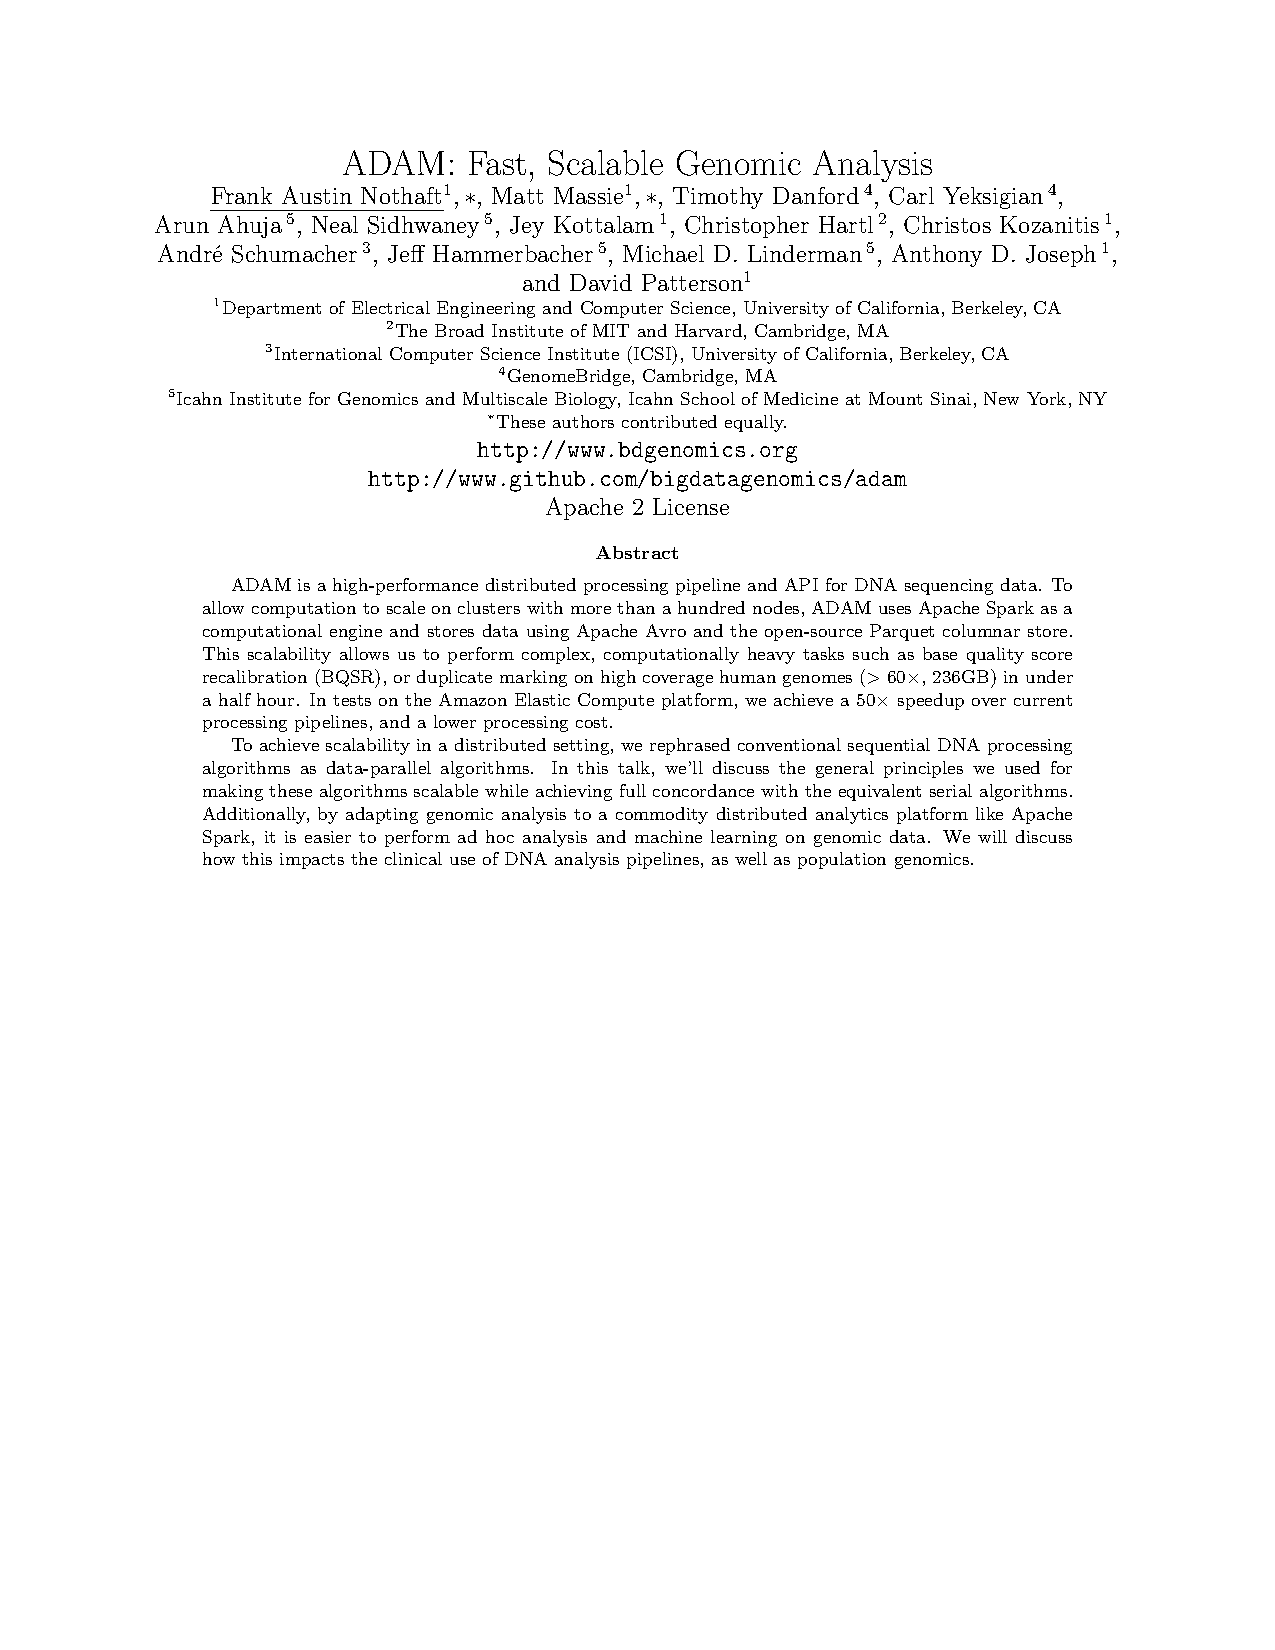
\includepdf[pages={1}]{GenomeScale-16-ADAM.pdf}
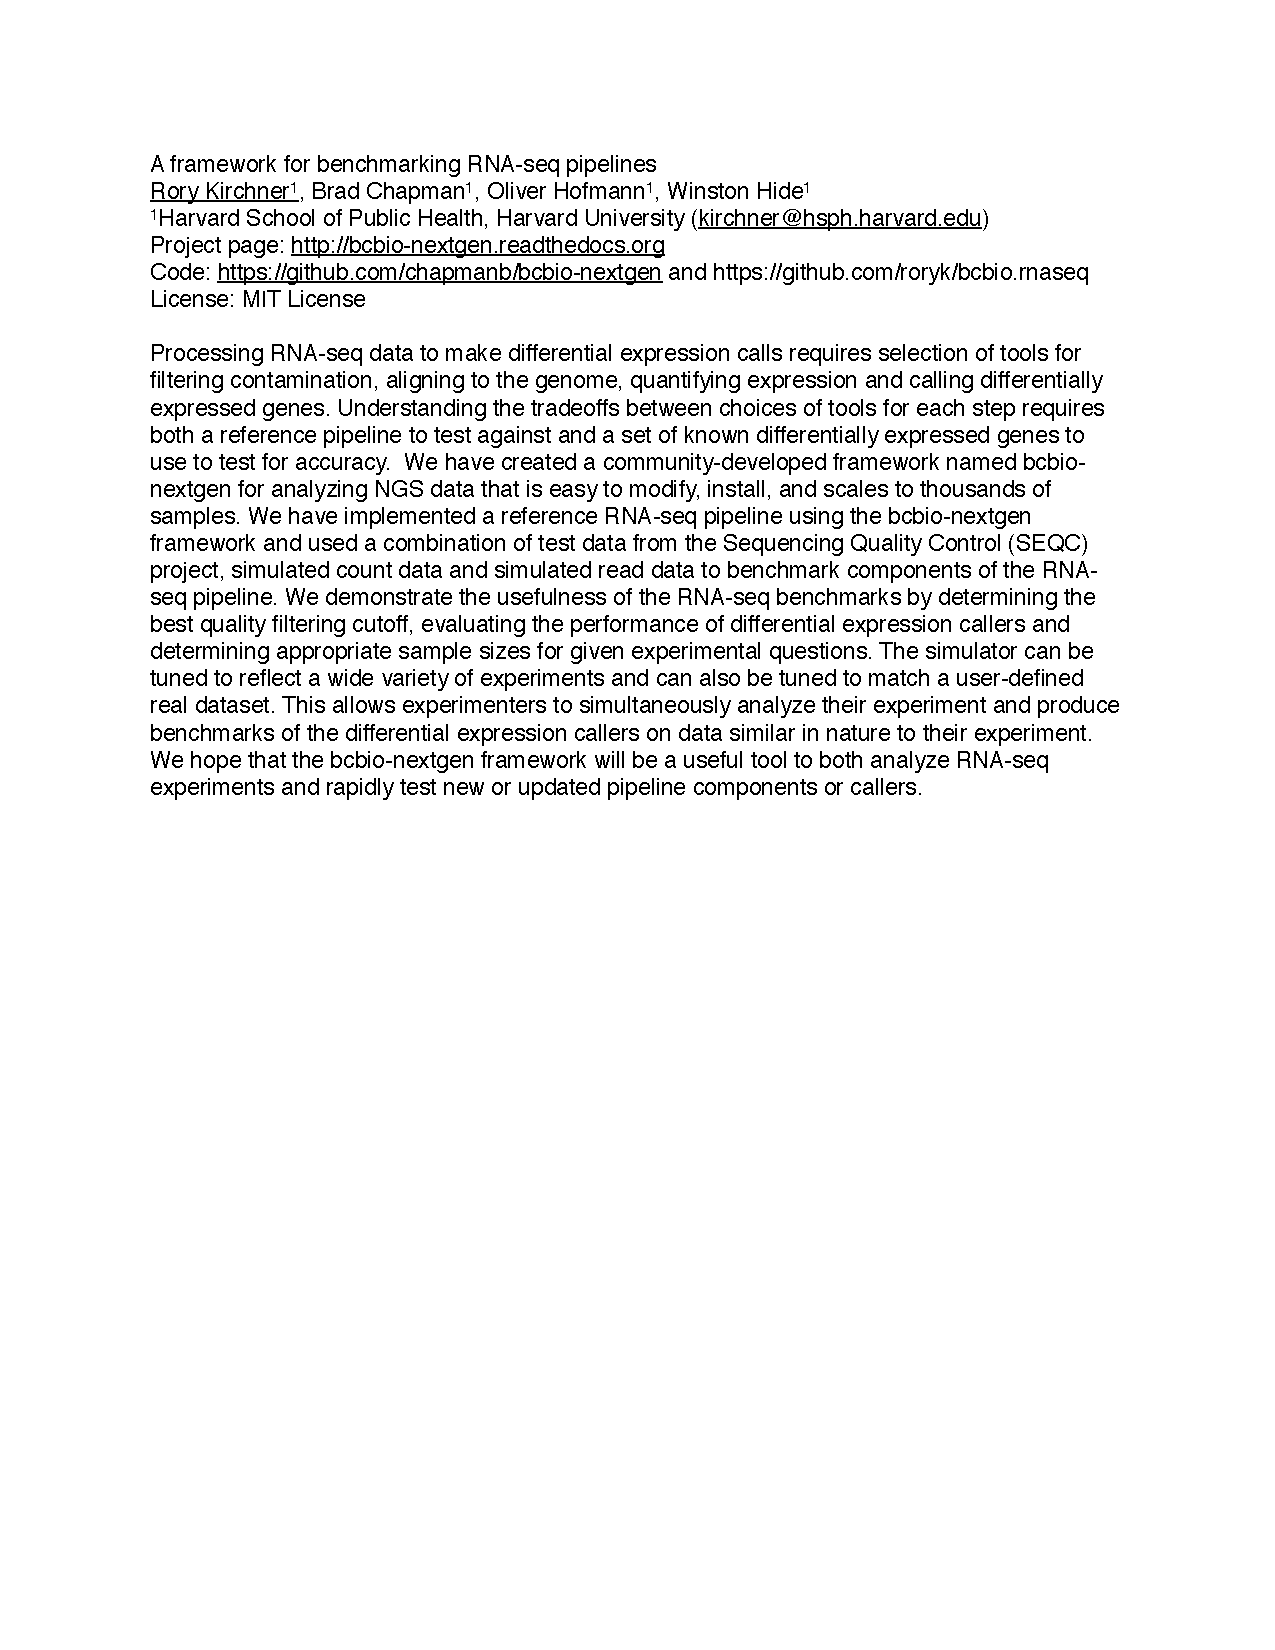
\includepdf[pages={1}]{GenomeScale-32-Framework-RNASeq.pdf}
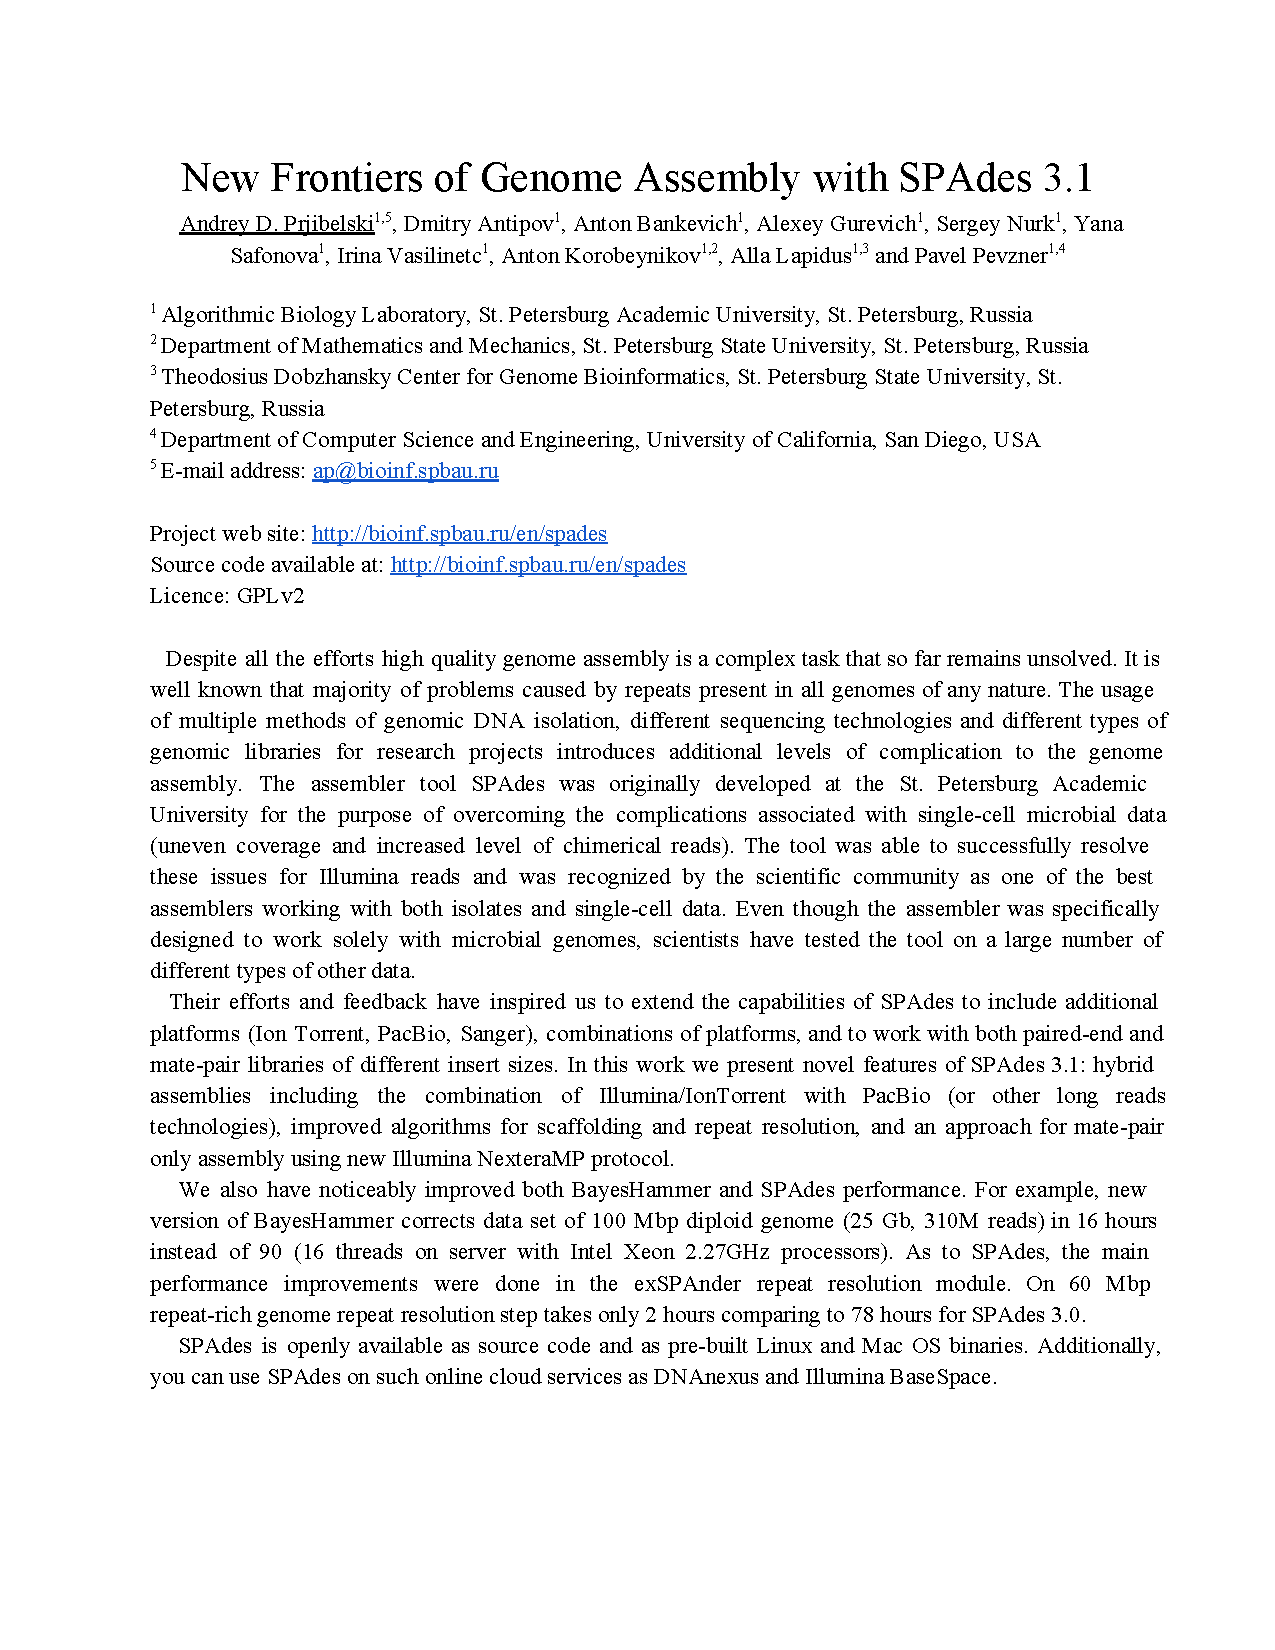
\includepdf[pages={1}]{GenomeScale-27-SPADES.pdf}
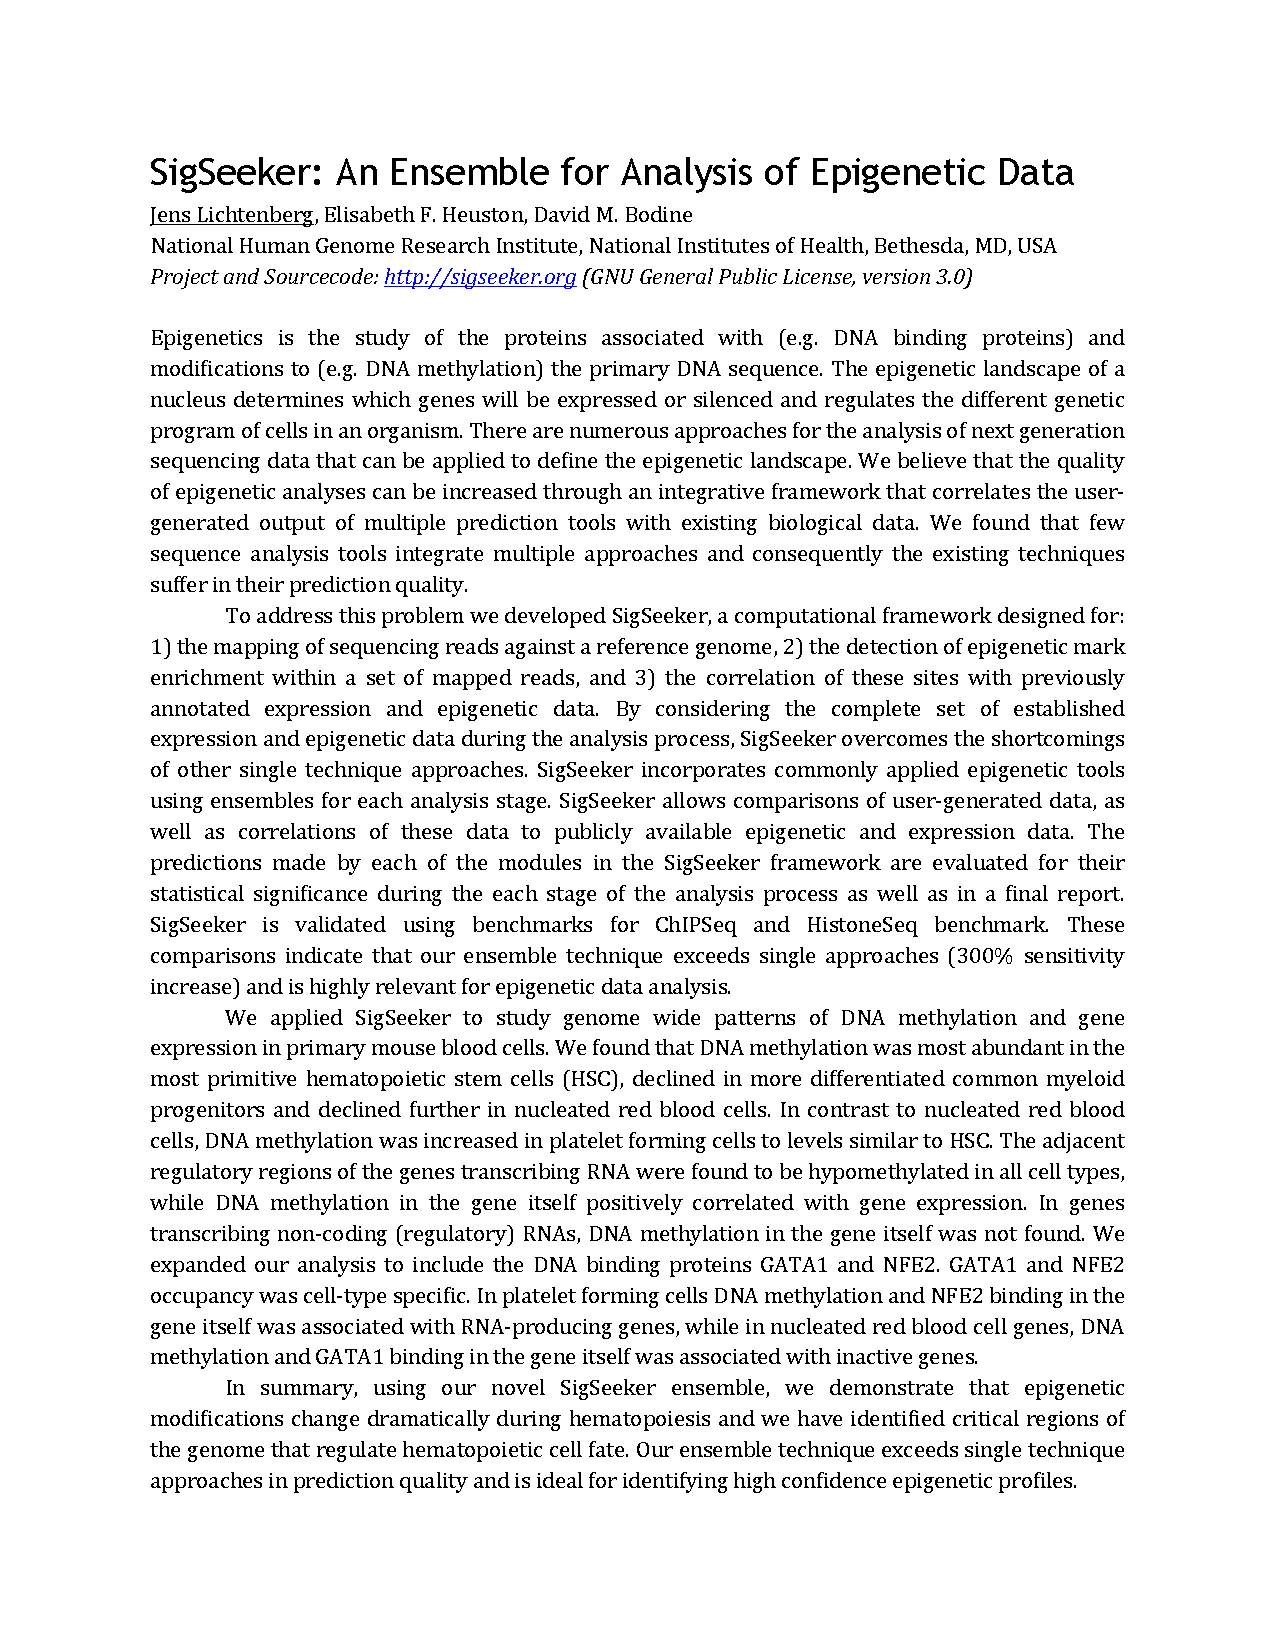
\includepdf[pages={1}]{GenomeScale-22-SigSeeker.pdf}
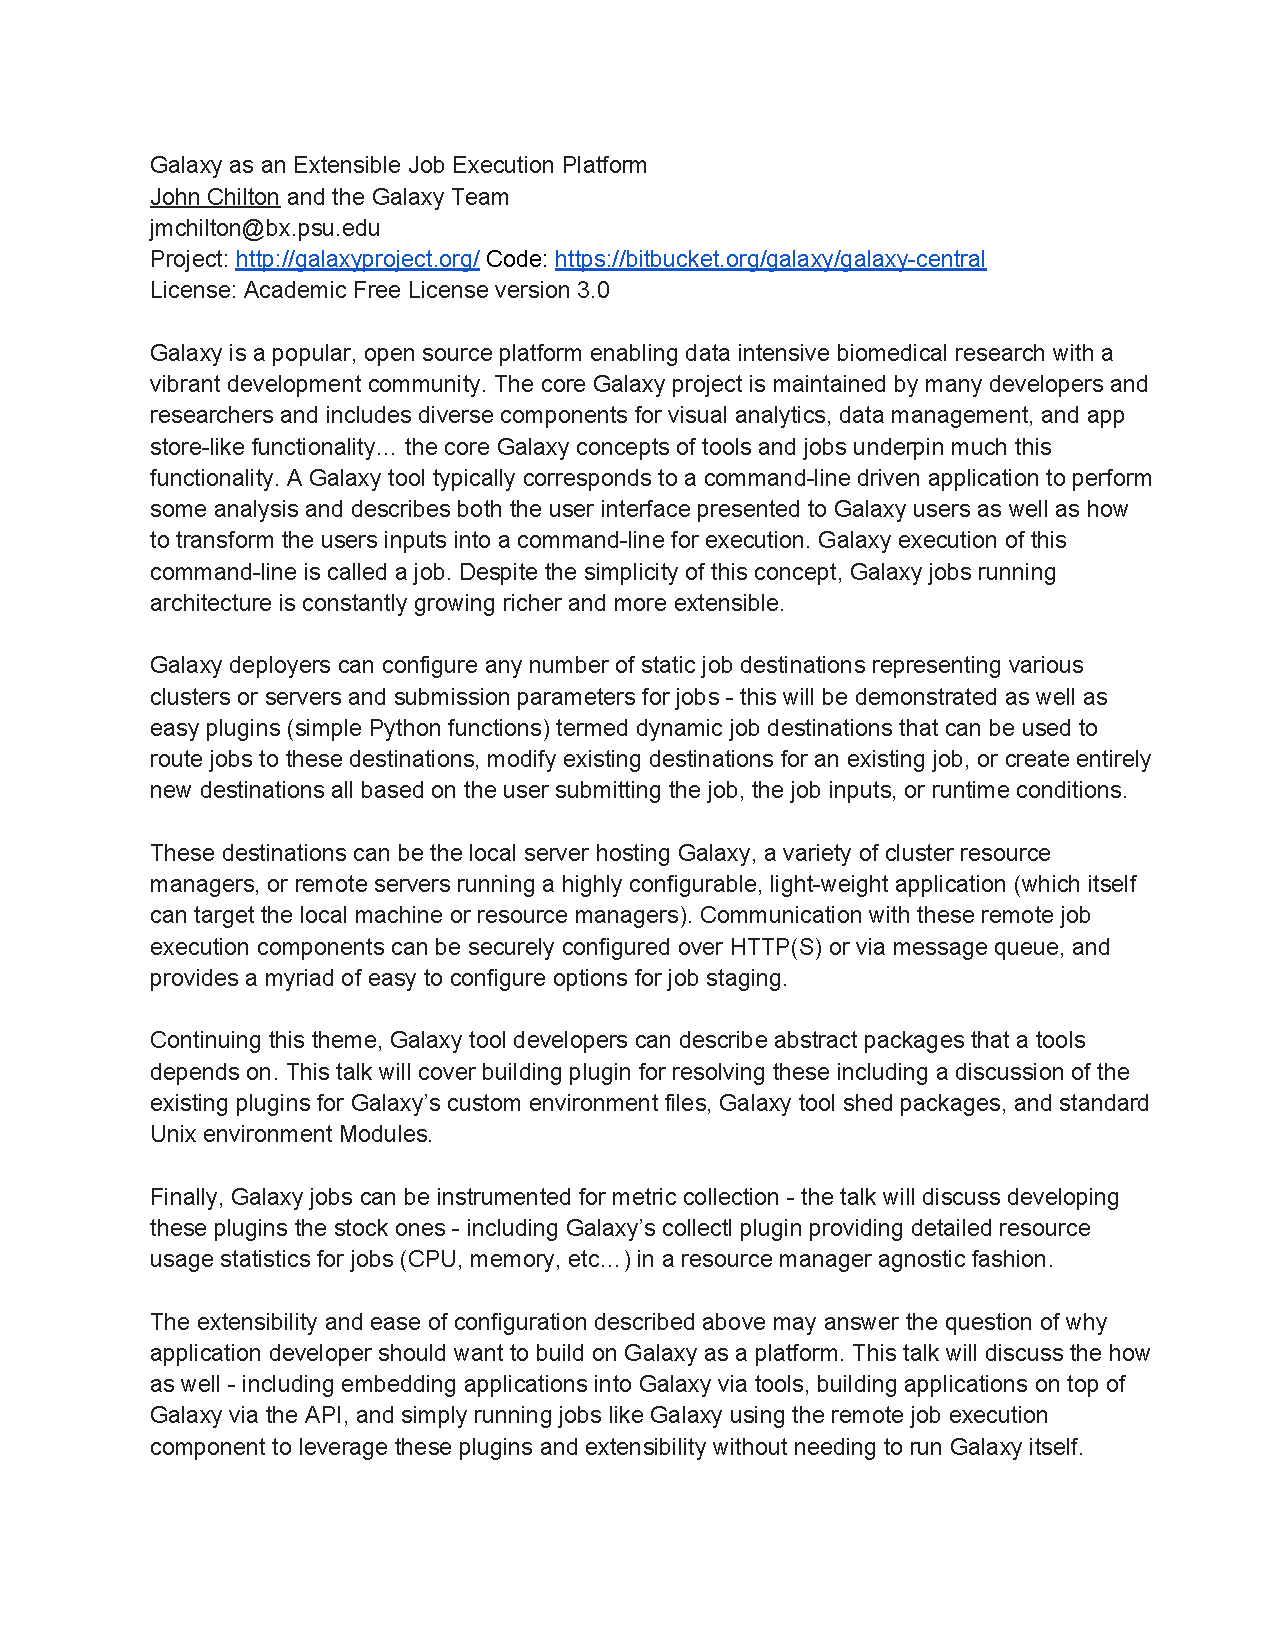
\includepdf[pages={1}]{GenomeScale-21-Galaxy-extending.pdf}

\newpage
\section*{Visualization}
BOSC 2014: Day One, 11 July 2014, afternoon session 14:00 -- 15:30. \\
\noindent Number of talks: Five (5) \\
\noindent Session chair: Rob Davey 
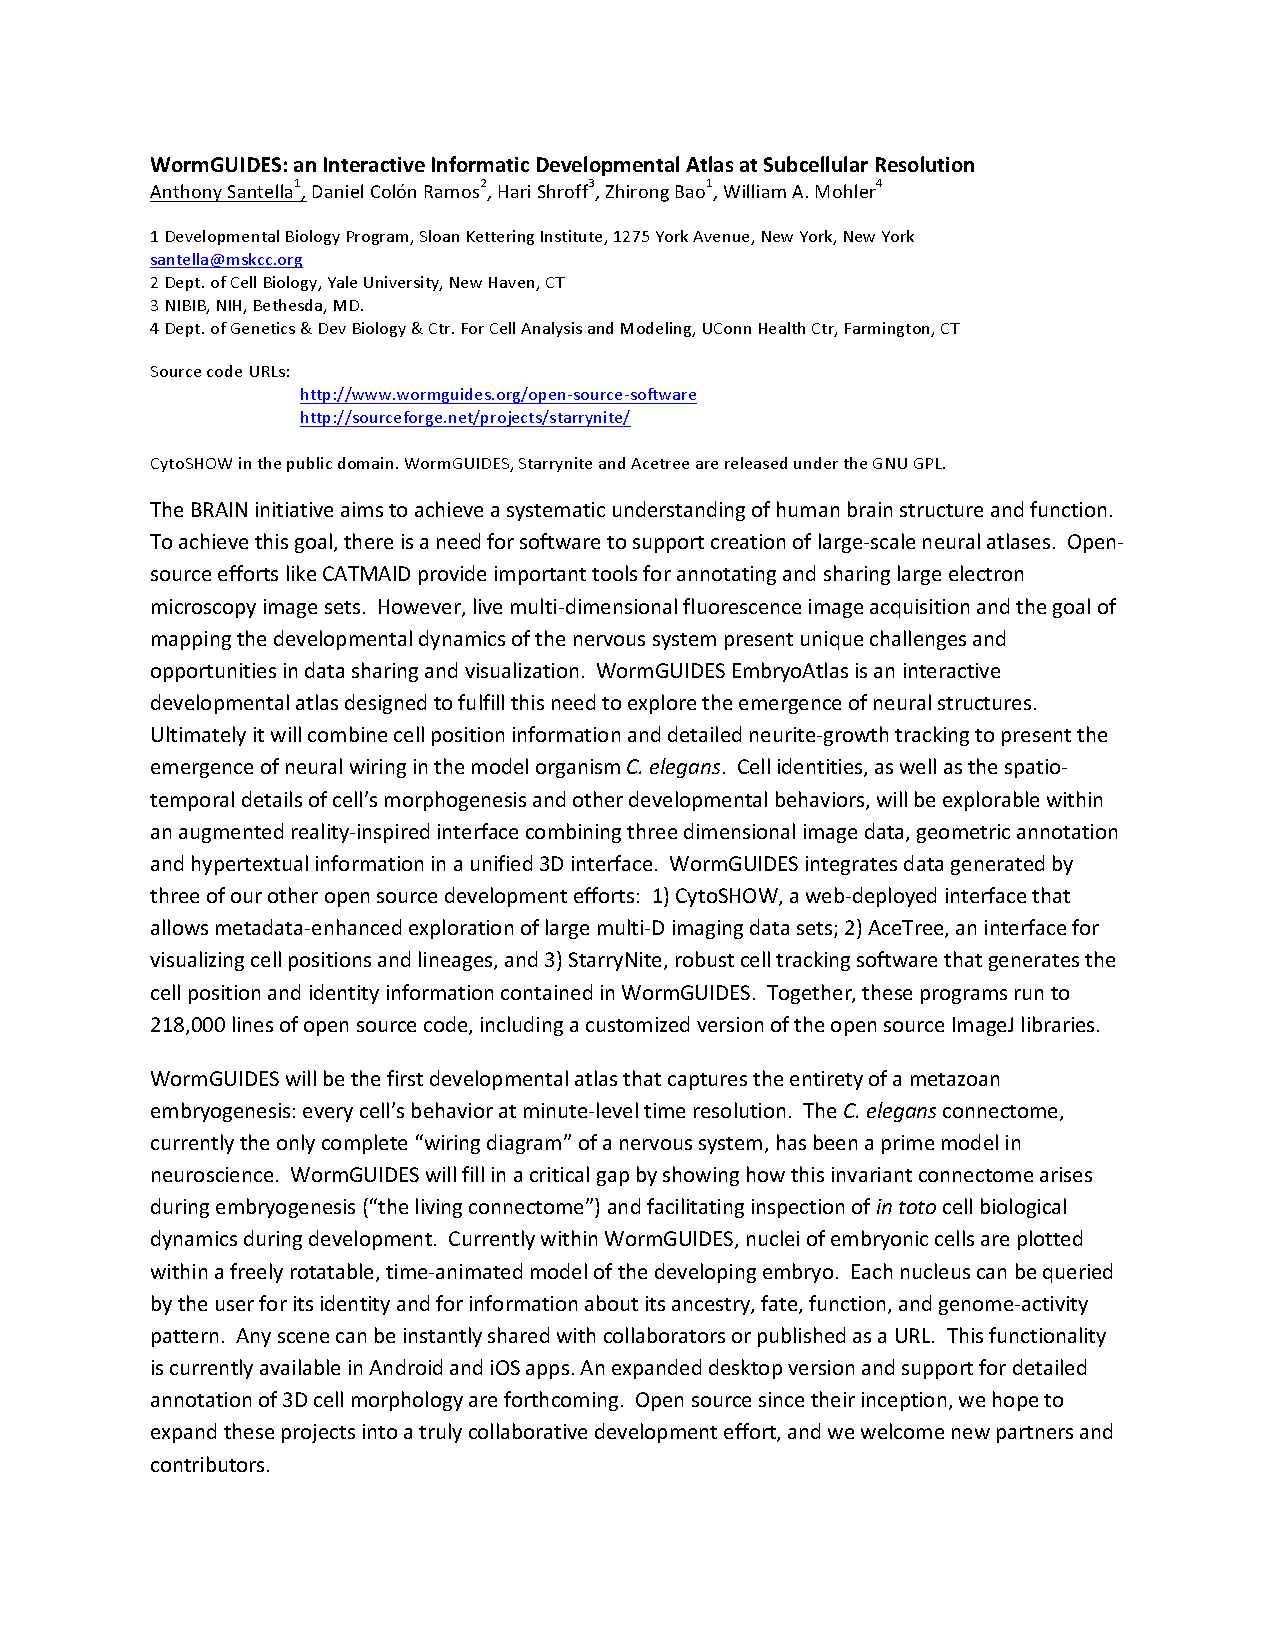
\includepdf[pages={1}]{Visualization-39-WormGUIDES.pdf}
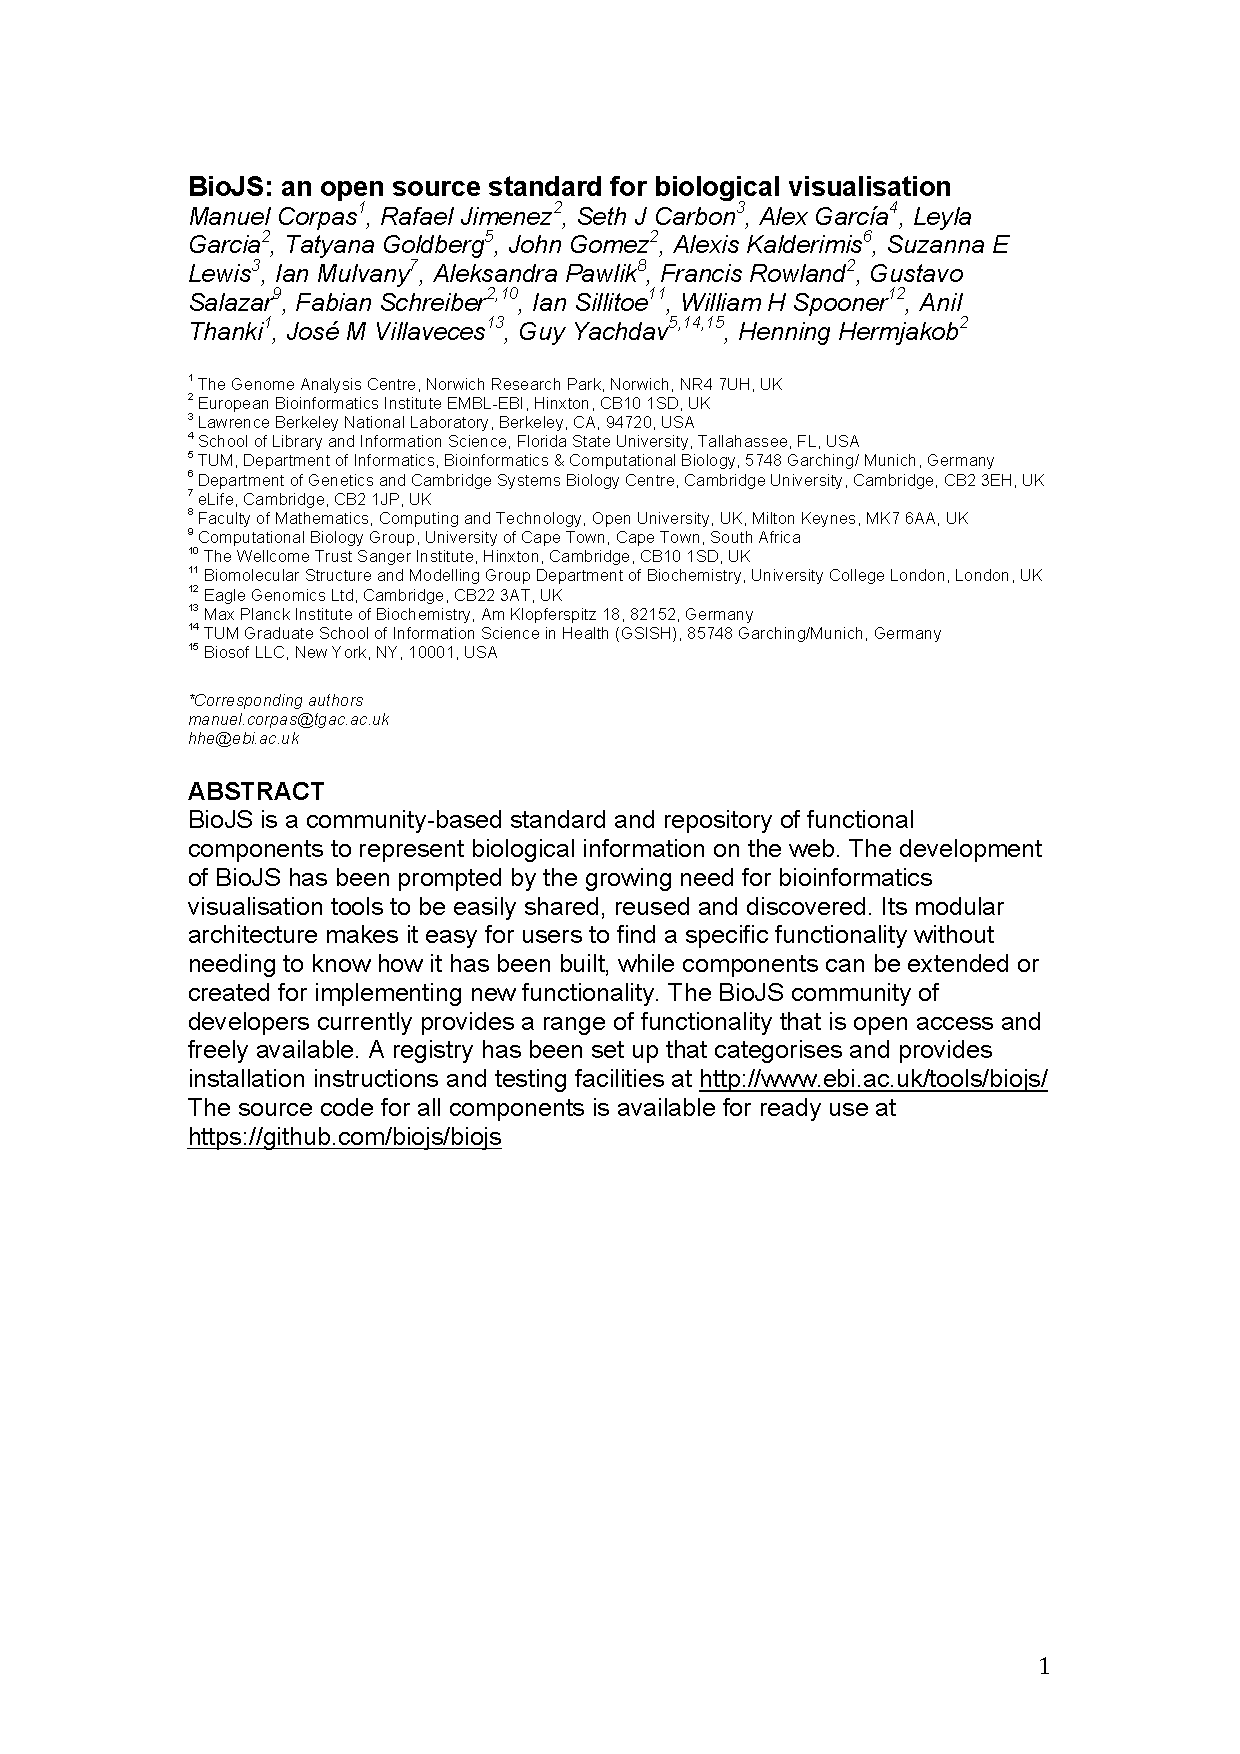
\includepdf[pages={1}]{Visualization-05-BioJS.pdf}
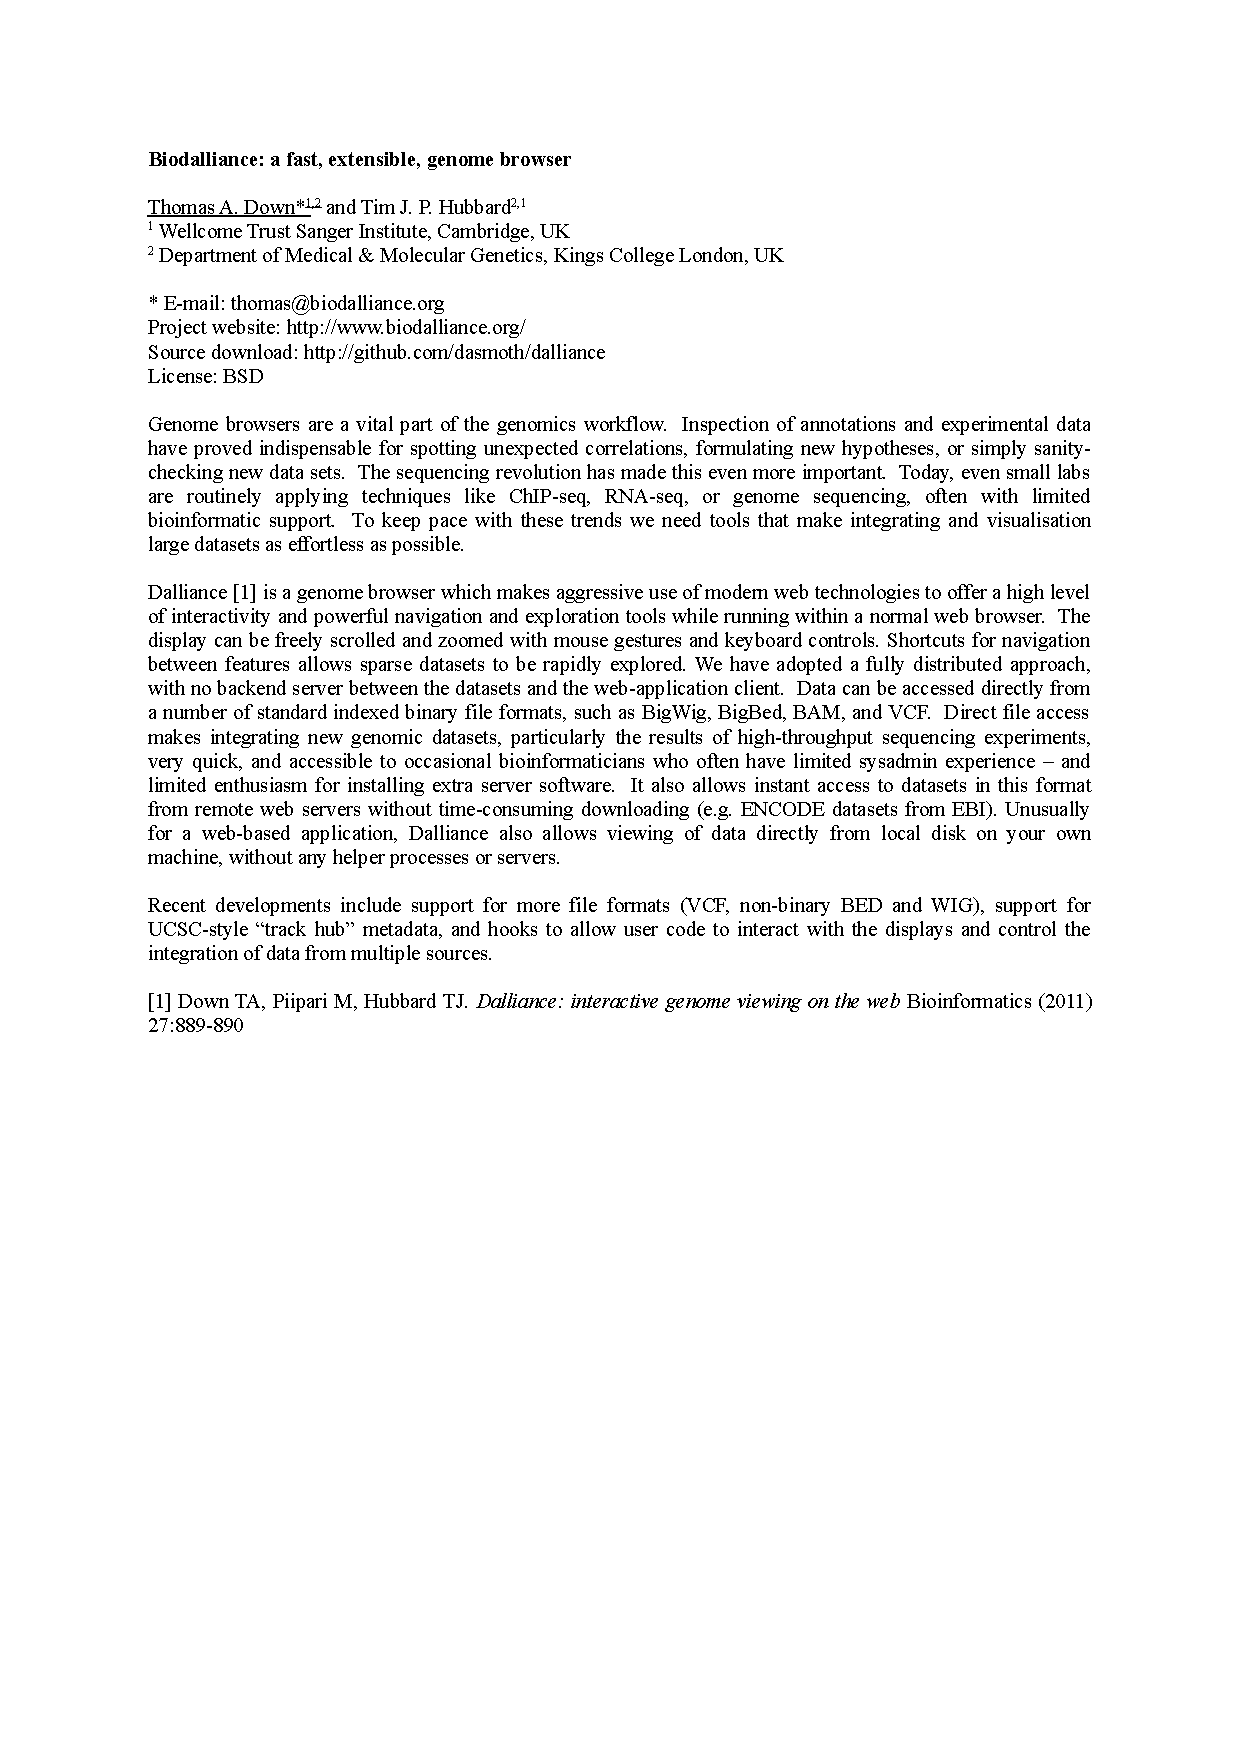
\includepdf[pages={1}]{Visualization-07-Biodalliance.pdf}
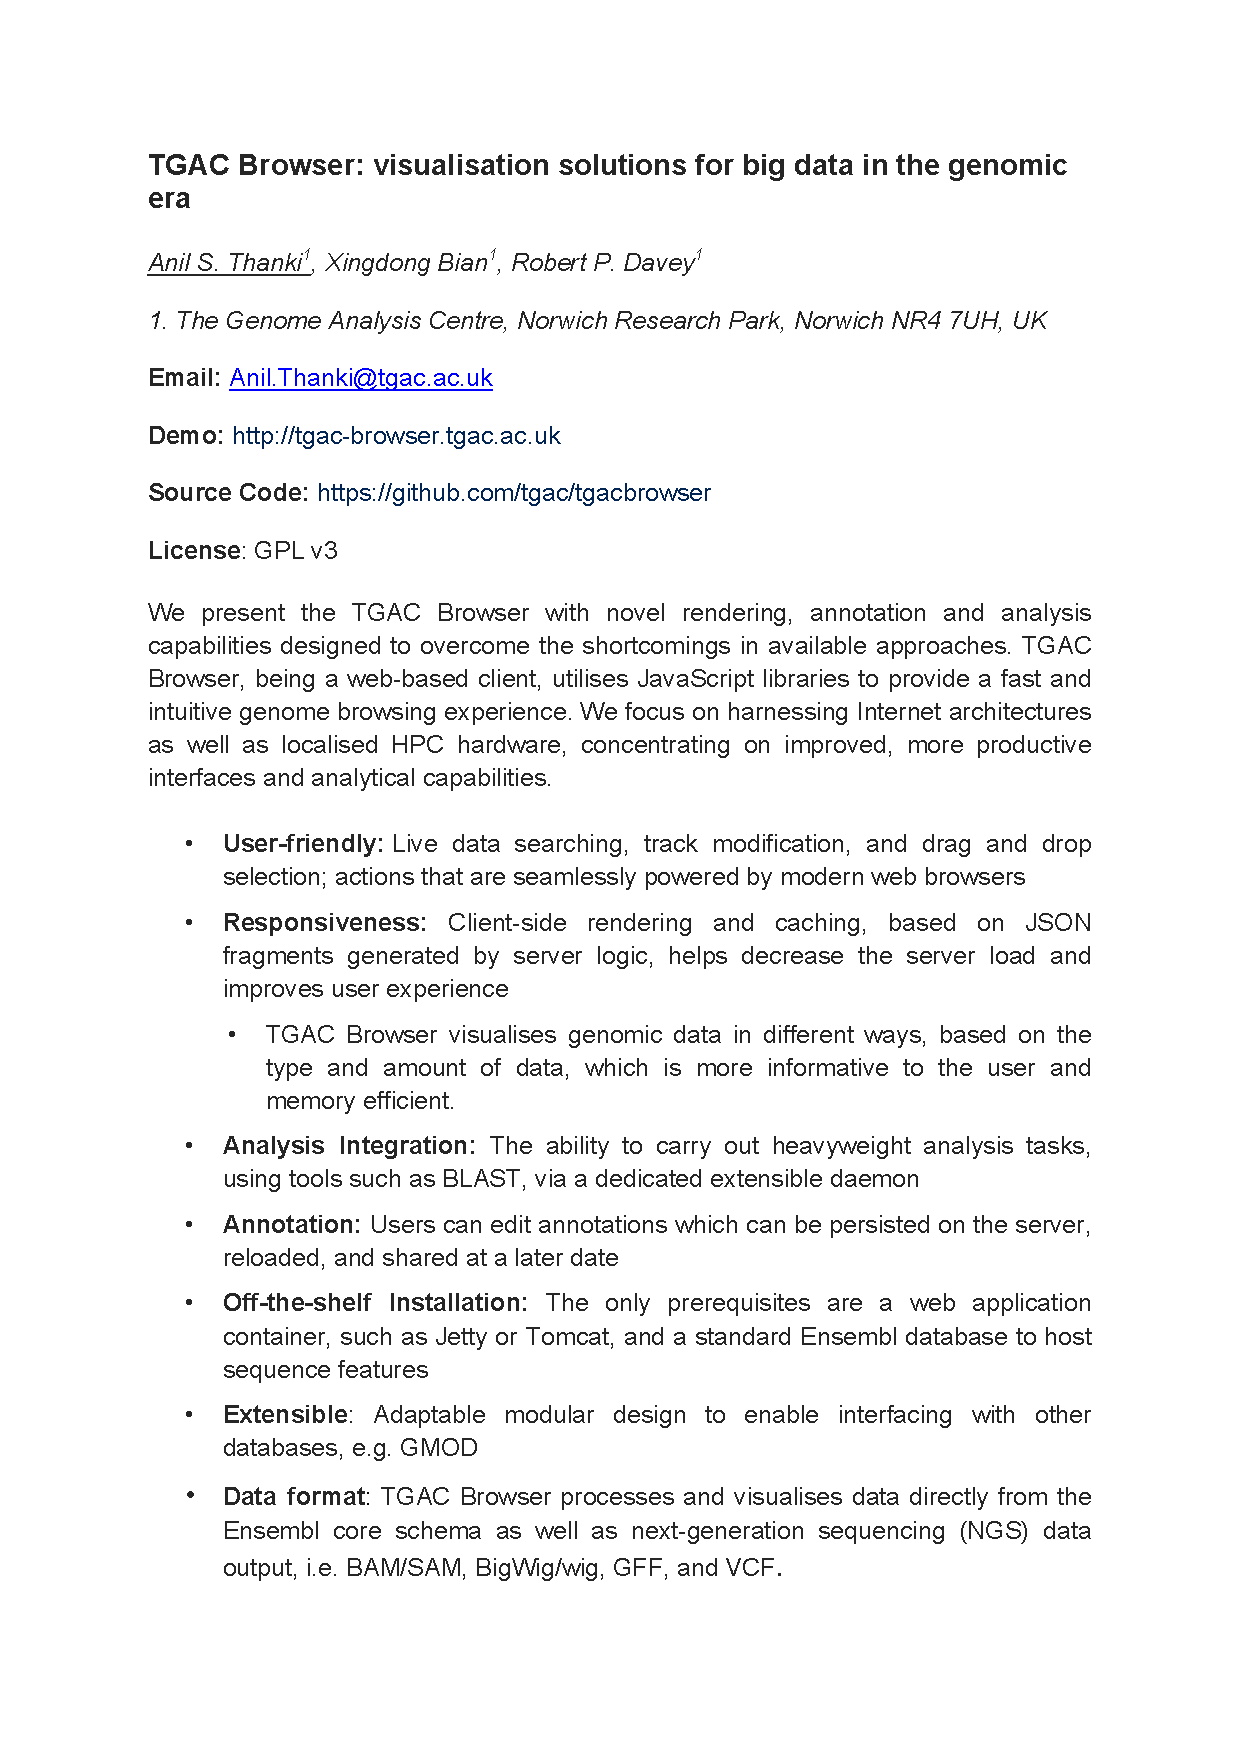
\includepdf[pages={1}]{Visualization-17-TGAC-browser.pdf}
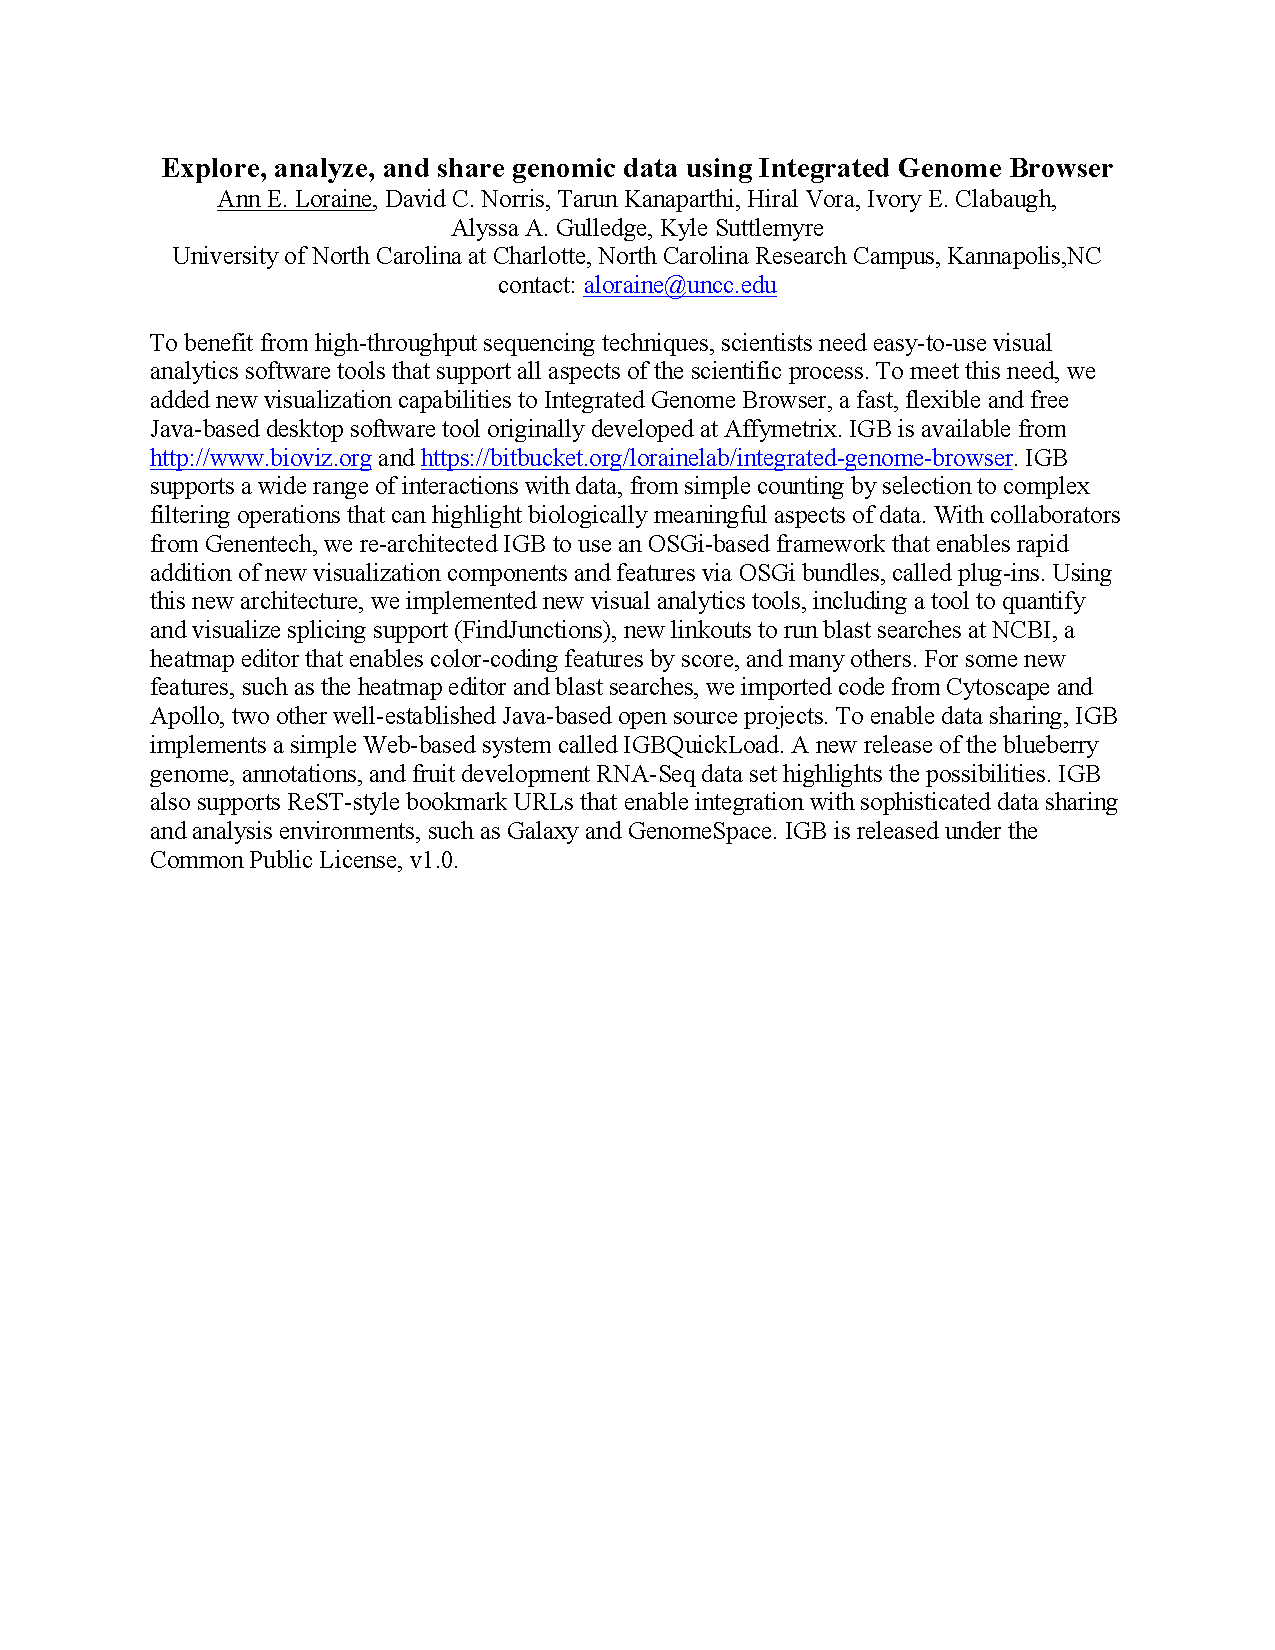
\includepdf[pages={1}]{Visualization-38-IGB.pdf}

\newpage
\section*{Bioinformatics Open Source Project Updates}
BOSC 2014: Day One, 11 July 2014, afternoon session 16:00 -- 17:00. \\
\noindent Number of talks: Five (5) \\
\noindent Session chair: Peter Cock 
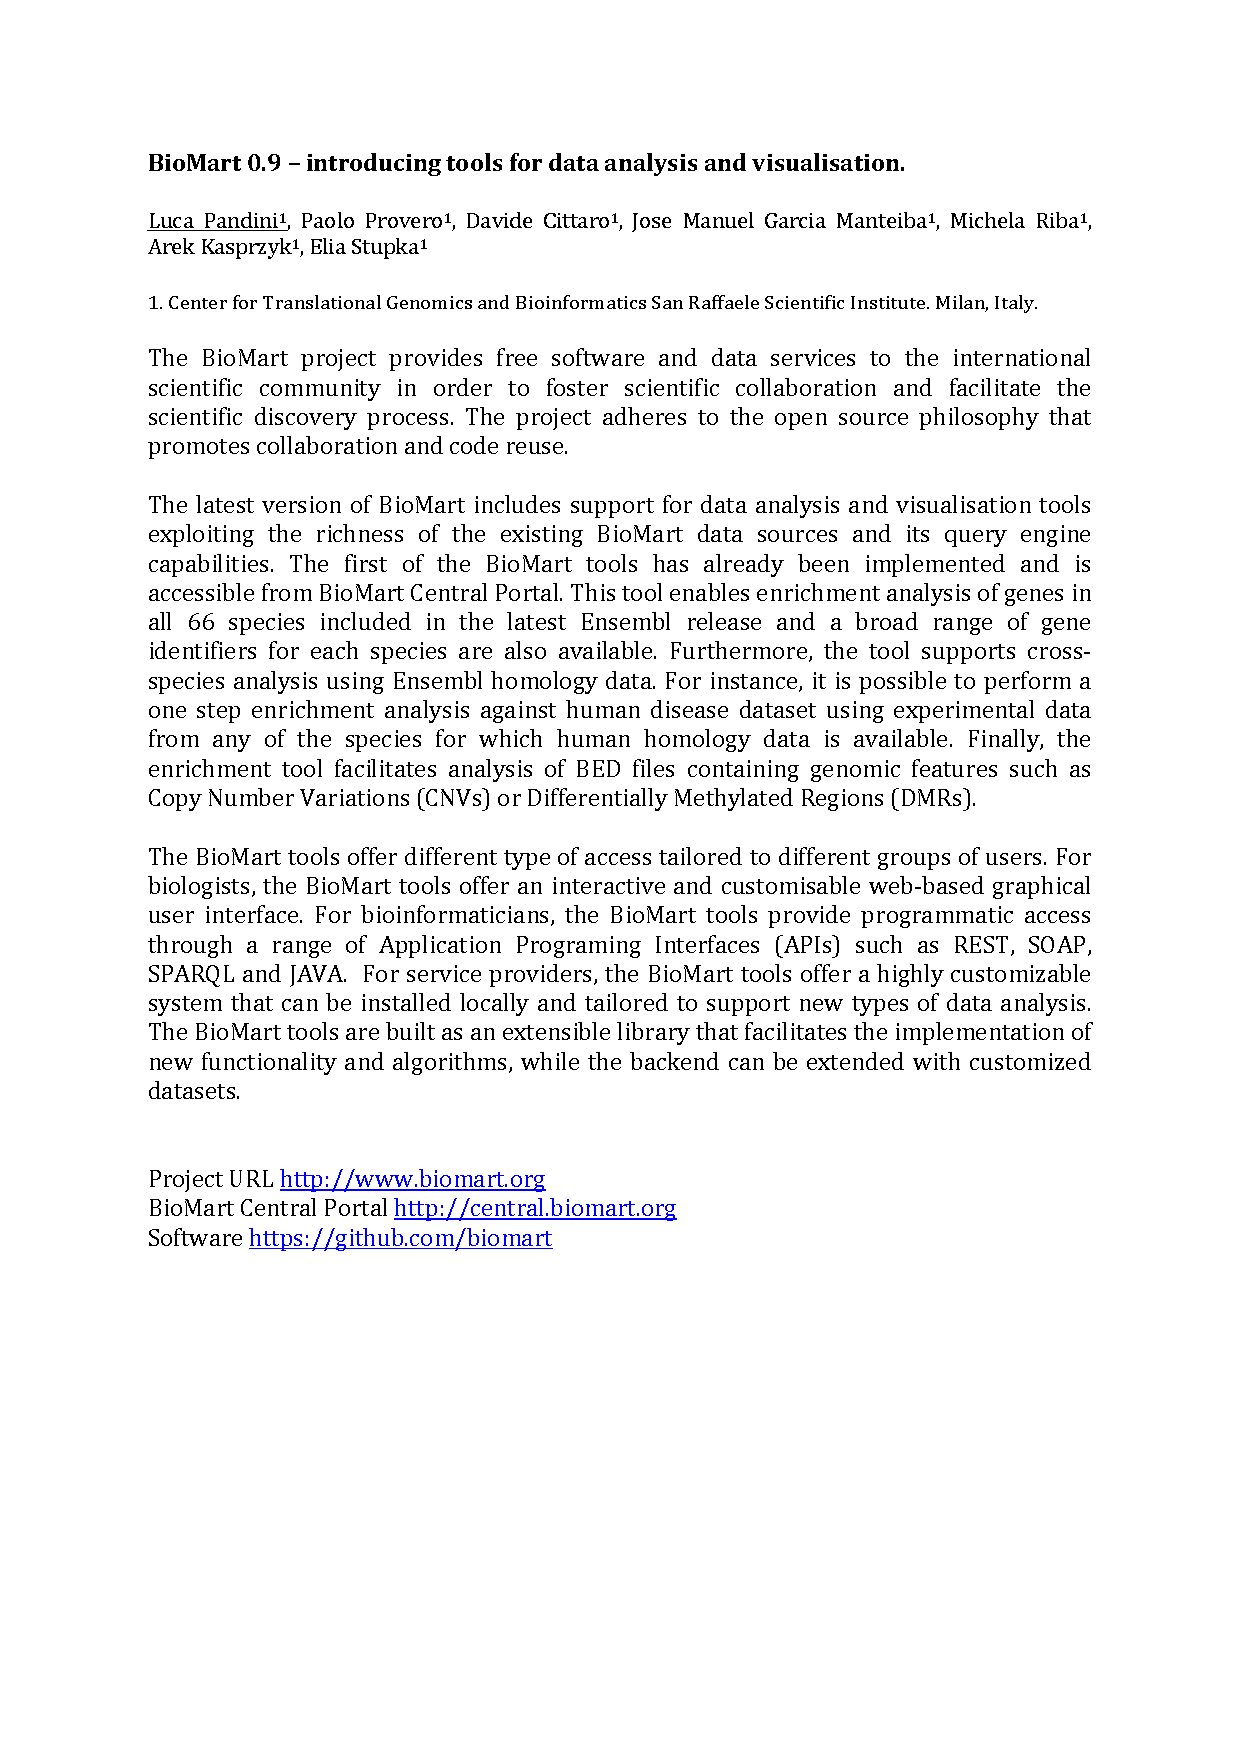
\includepdf[pages={1}]{Updates-20-BioMart.pdf}
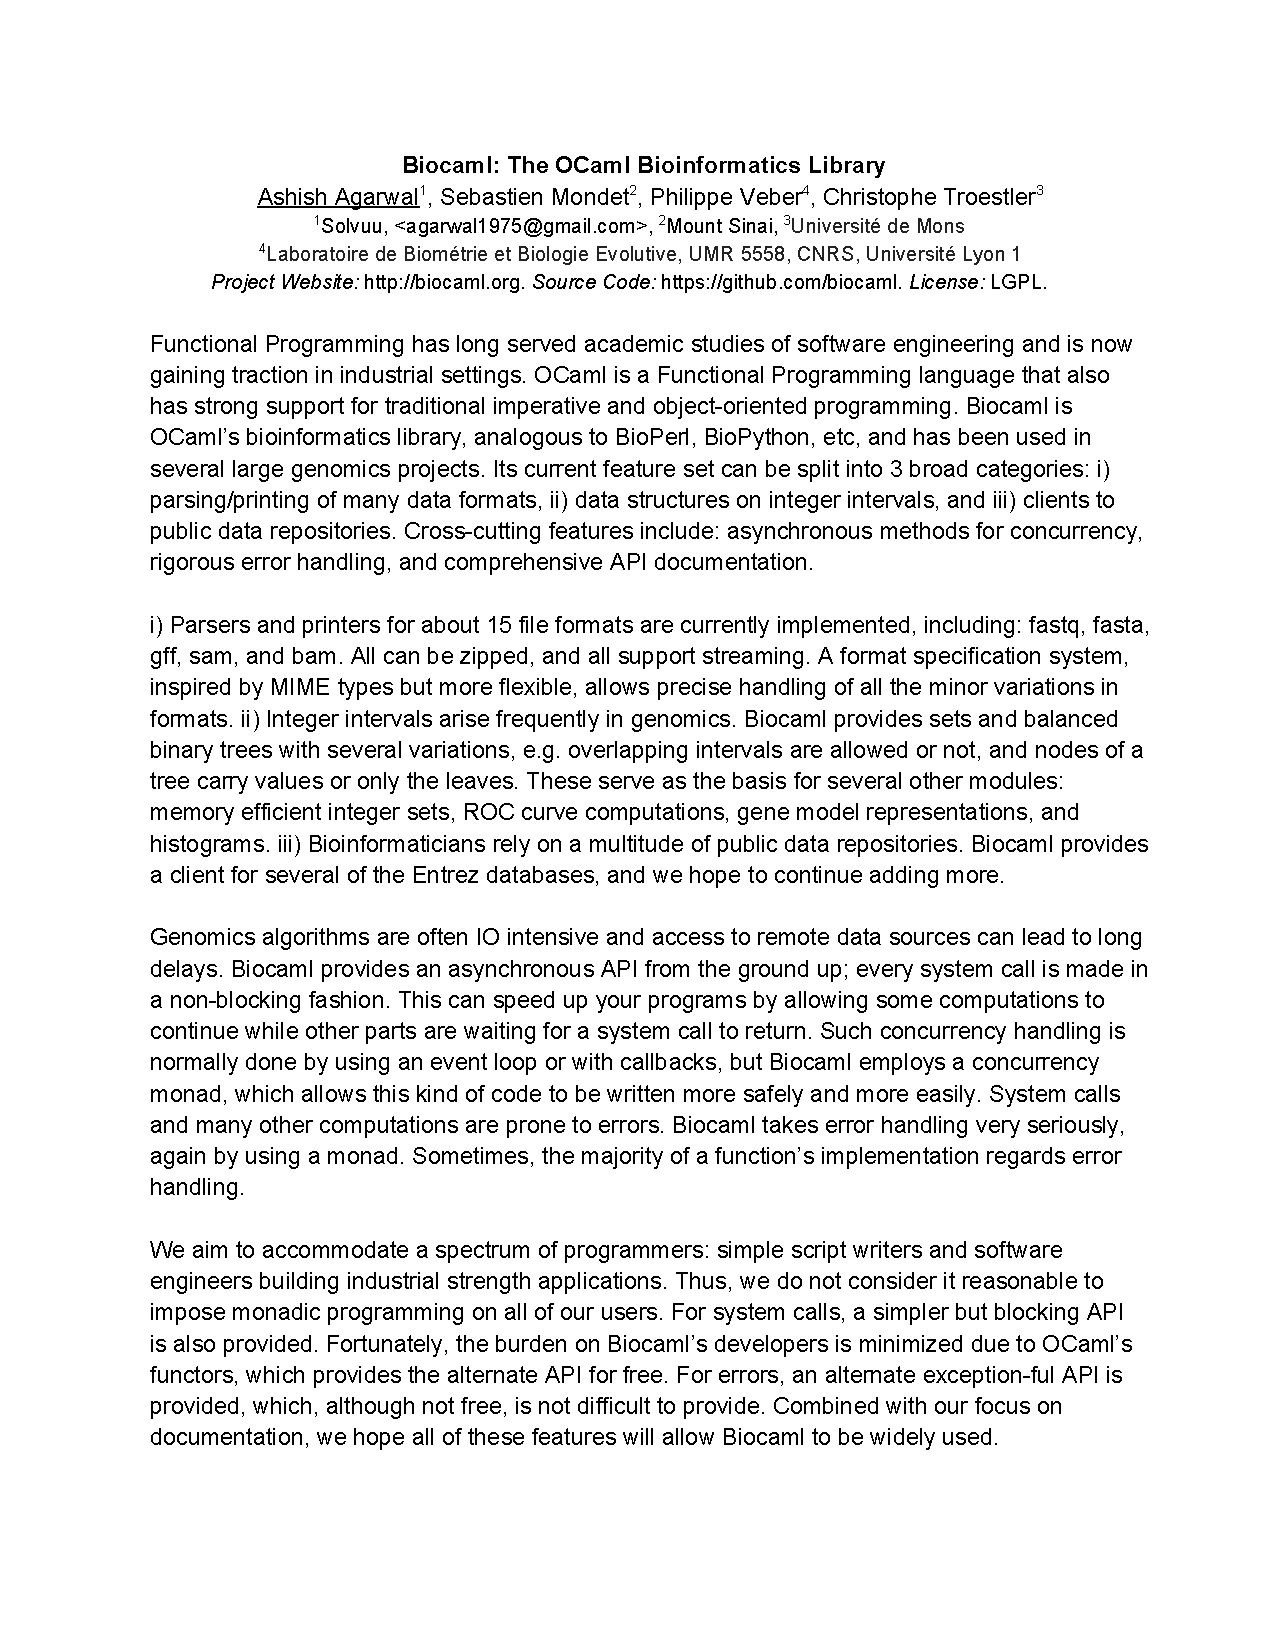
\includepdf[pages={1}]{Updates-25-Biocaml.pdf}
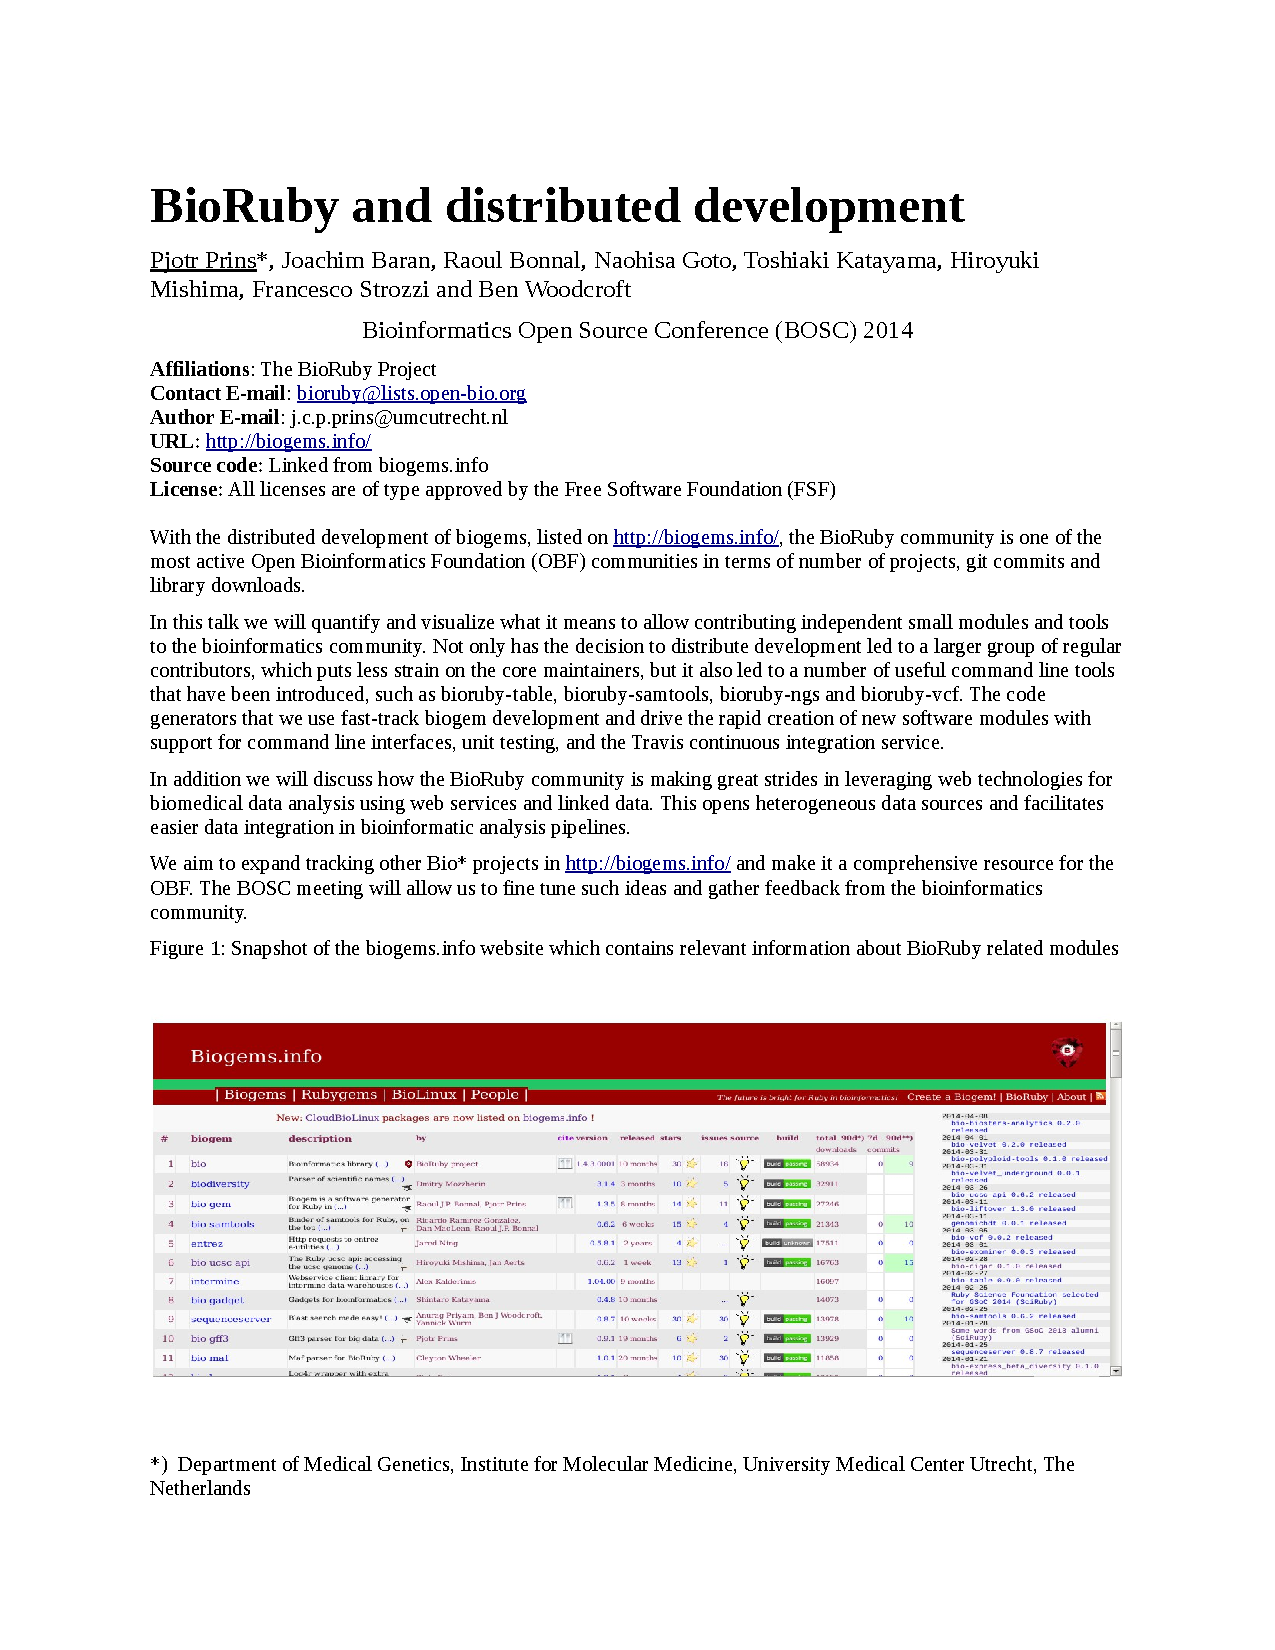
\includepdf[pages={1}]{Updates-41-BioRuby.pdf}
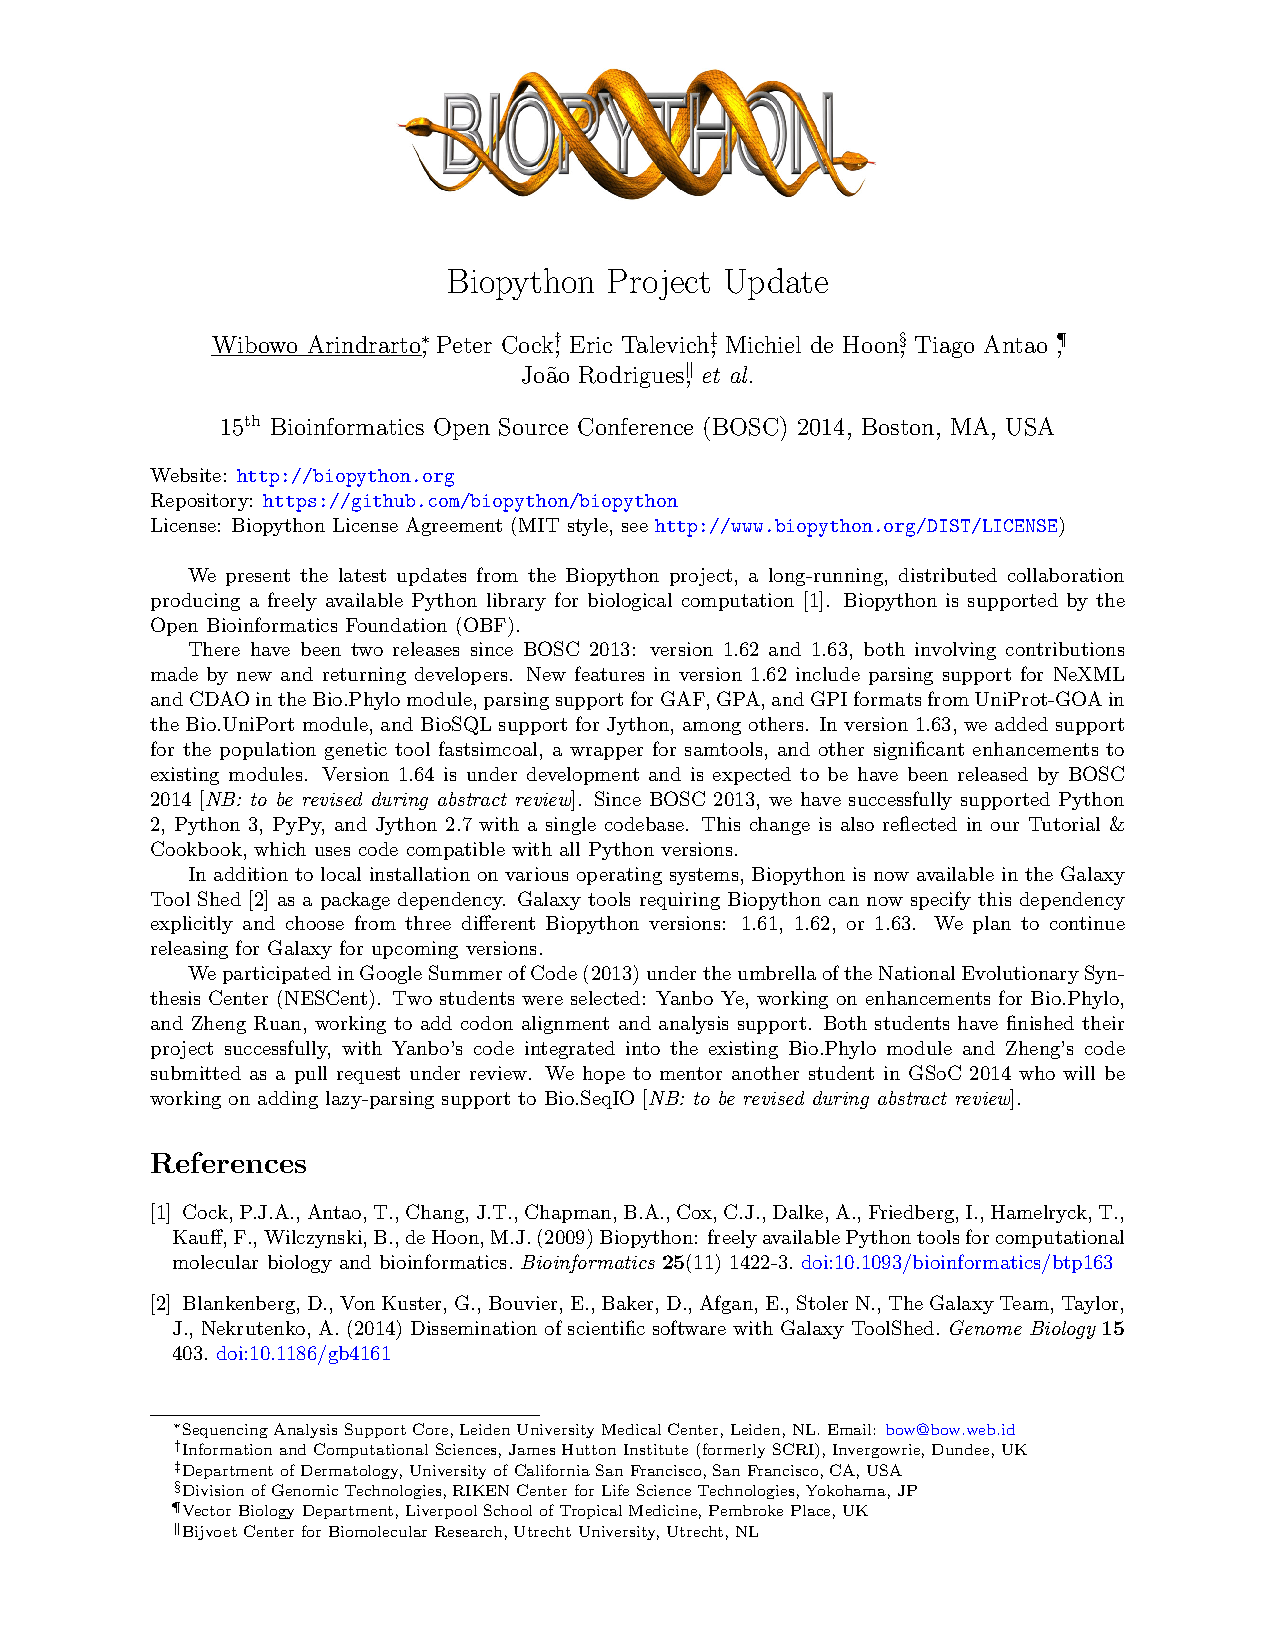
\includepdf[pages={1}]{Updates-19-Biopython.pdf}
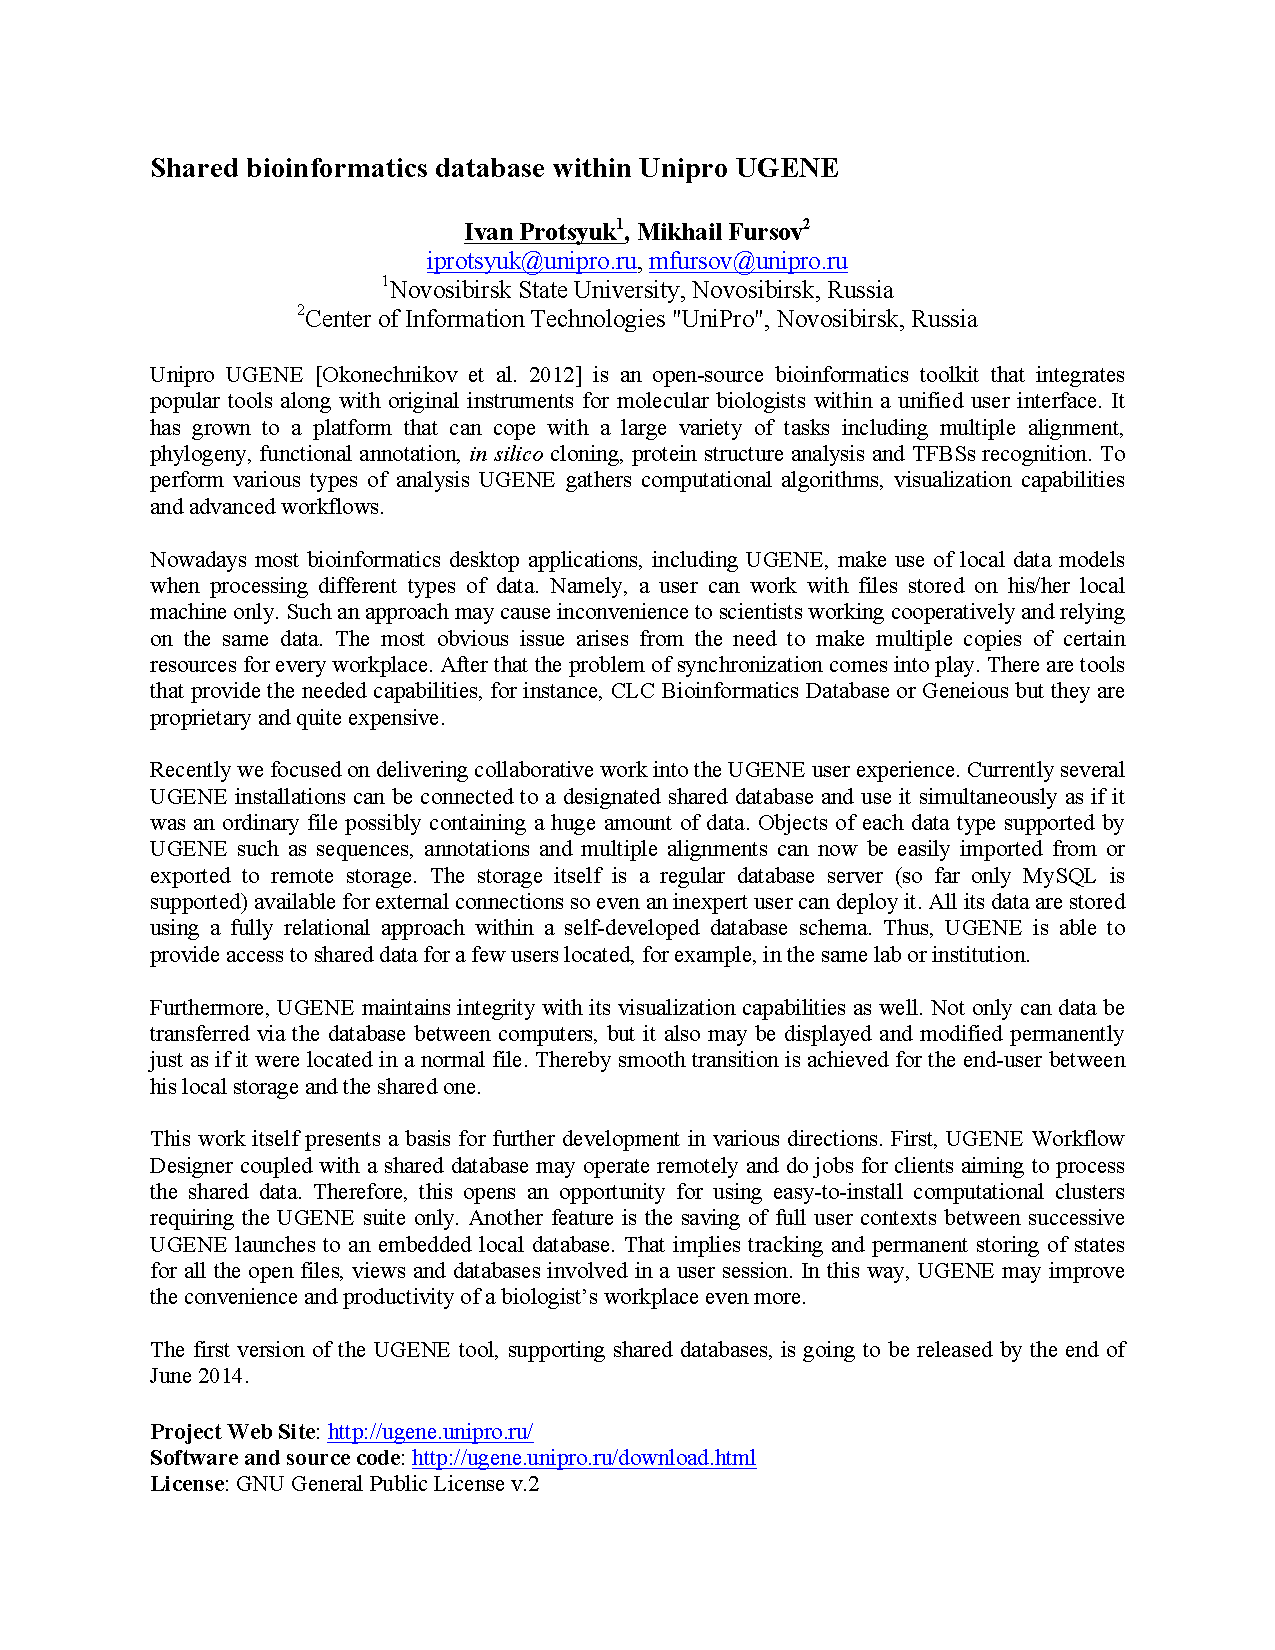
\includepdf[pages={1}]{Updates-02-UGENE.pdf}

\newpage
\section*{Software Interoperability}
BOSC 2014: Day Two, 12 July 2014, morning session 10:45 -- 12:30. \\
\noindent Number of talks: Five (5) \\
\noindent Session chair: Raoul Bonnal 
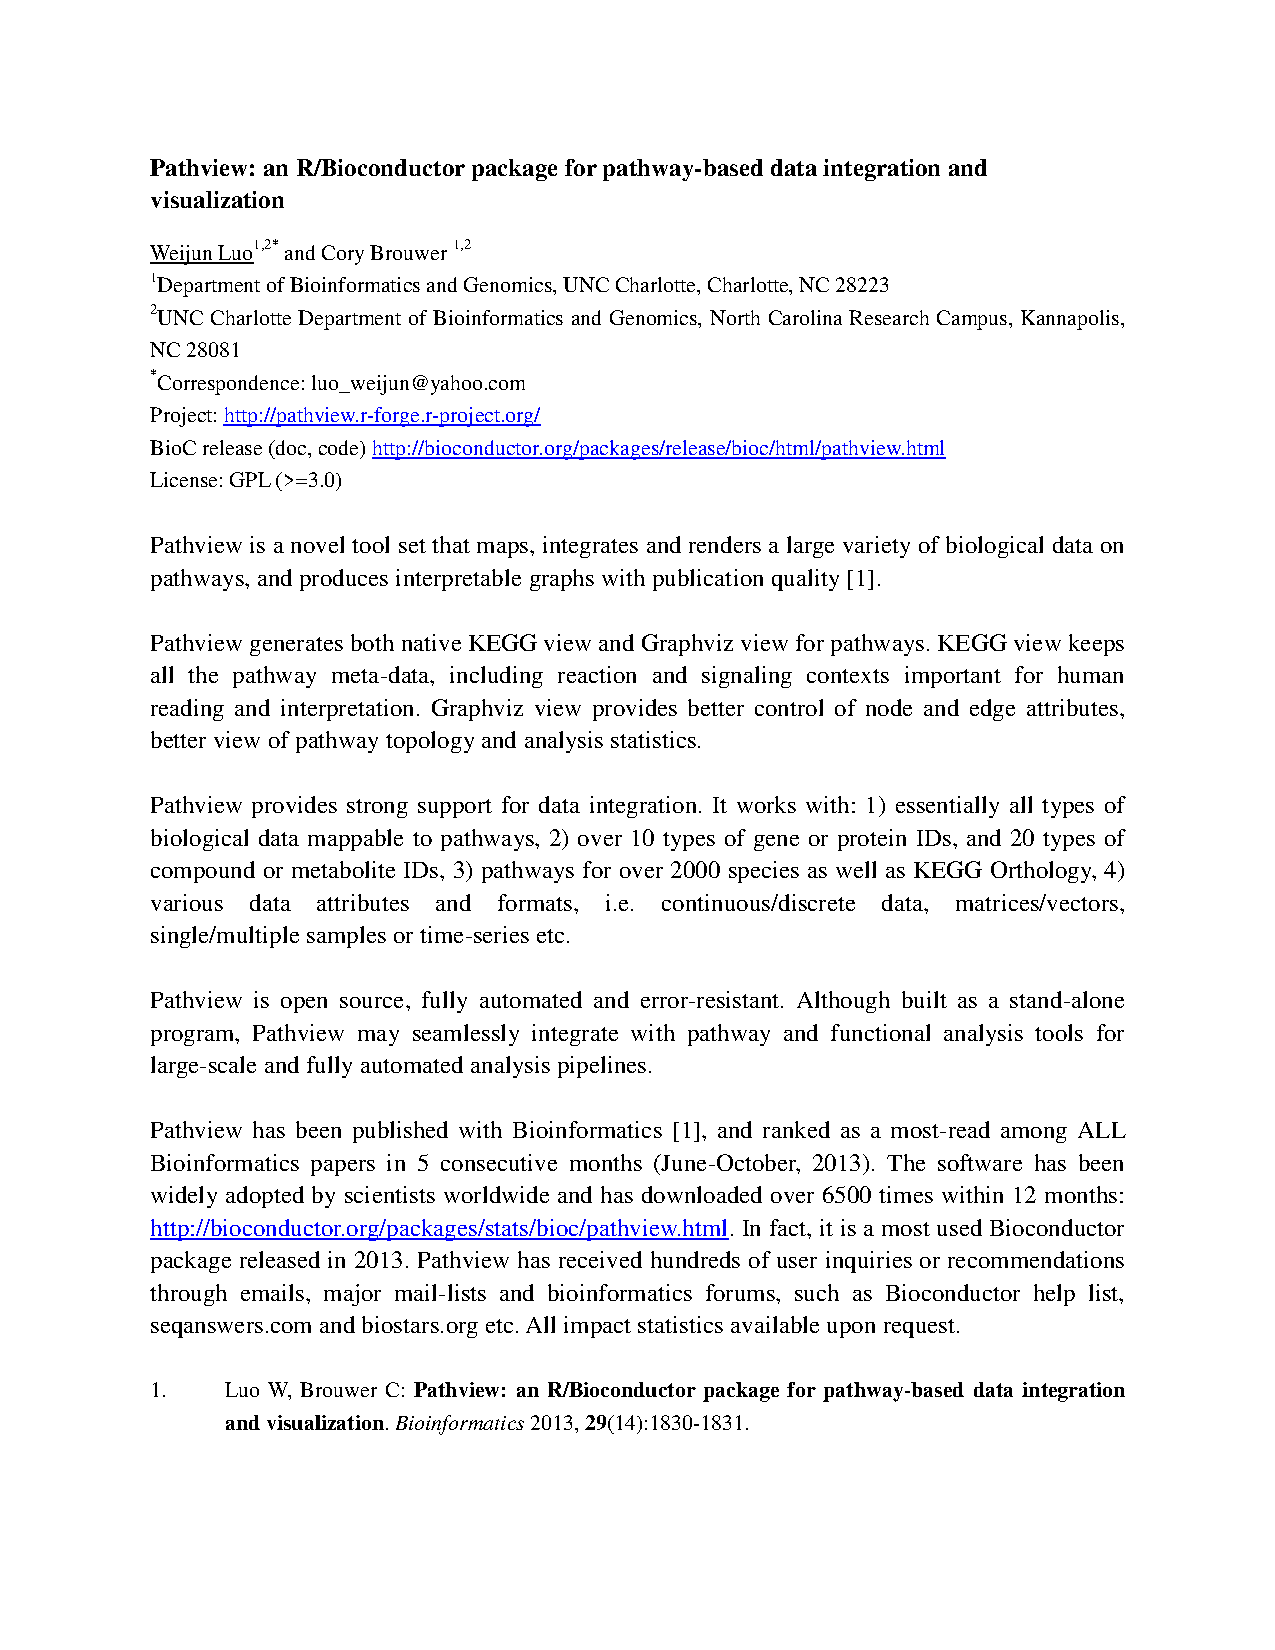
\includepdf[pages={1}]{Interoperability-04-Pathview.pdf}
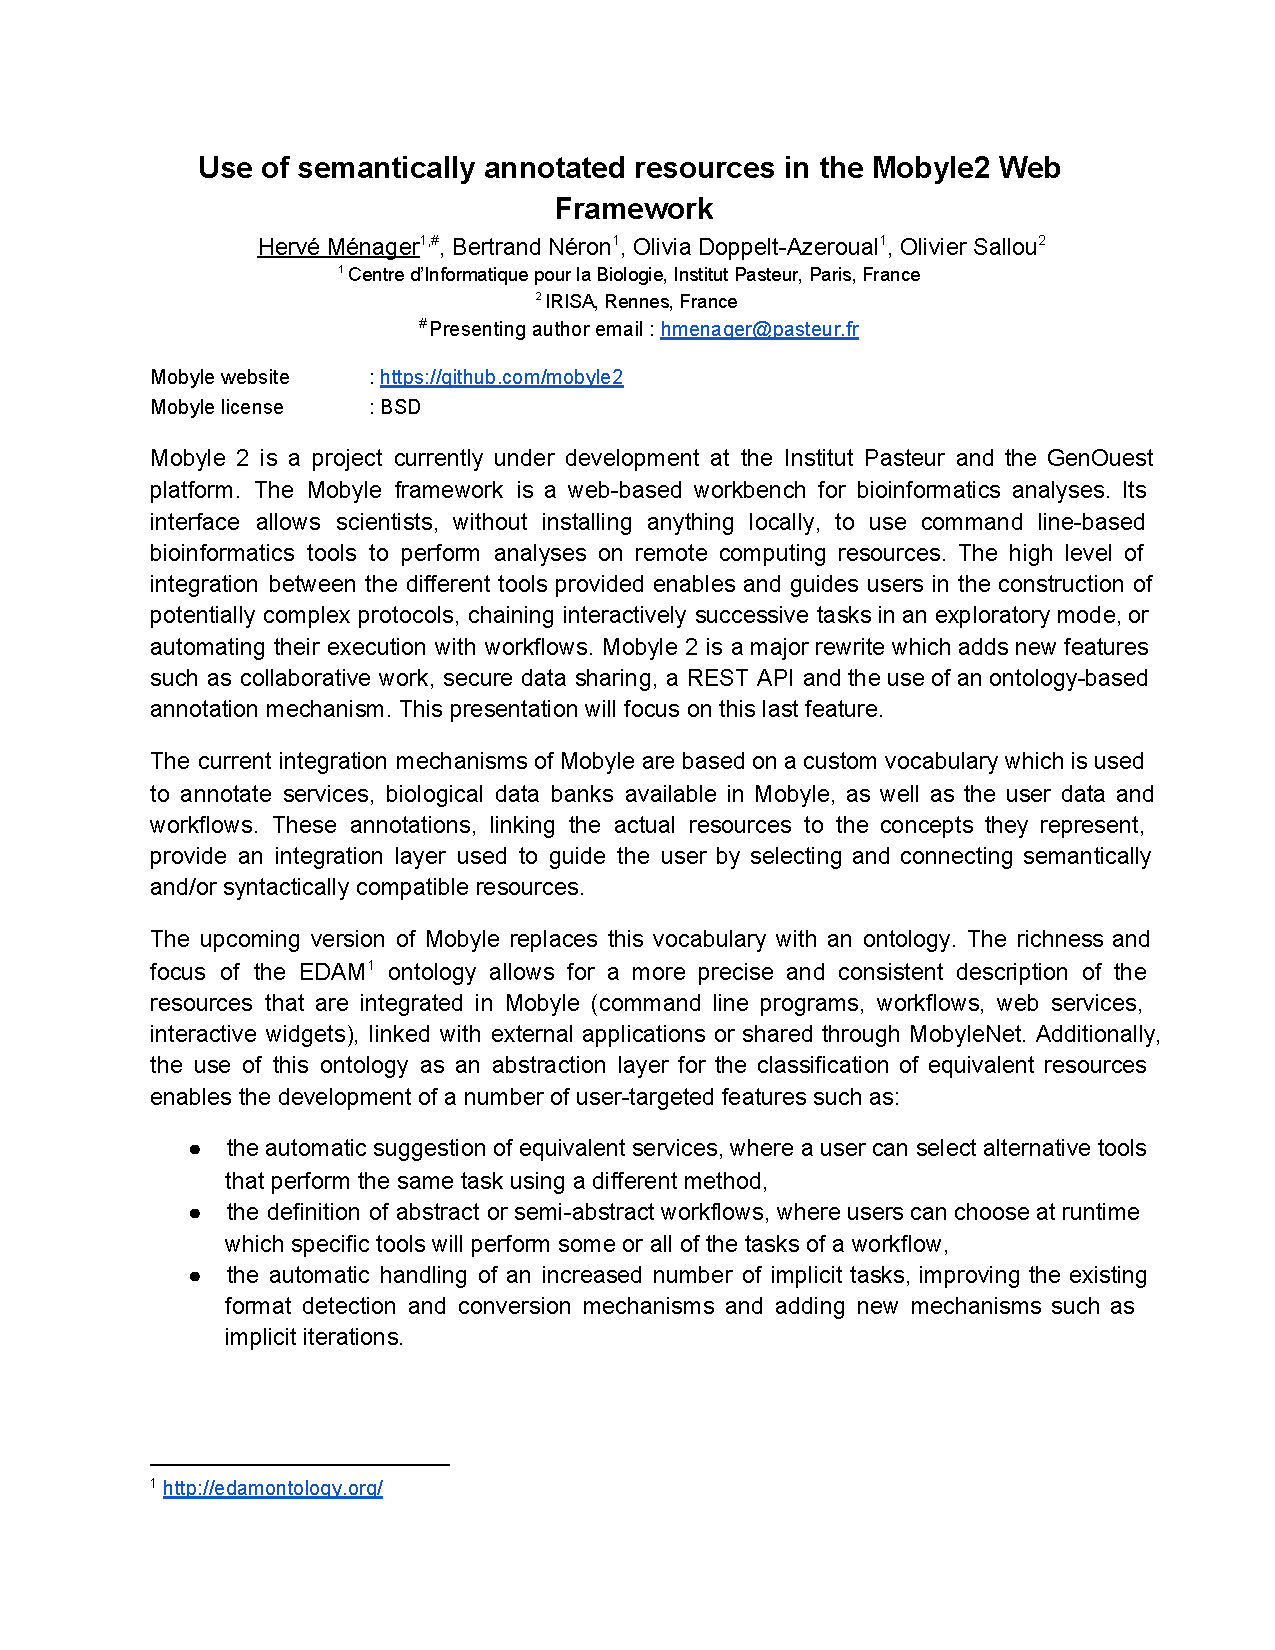
\includepdf[pages={1}]{Ineroperability-13-Mobyle2.pdf}
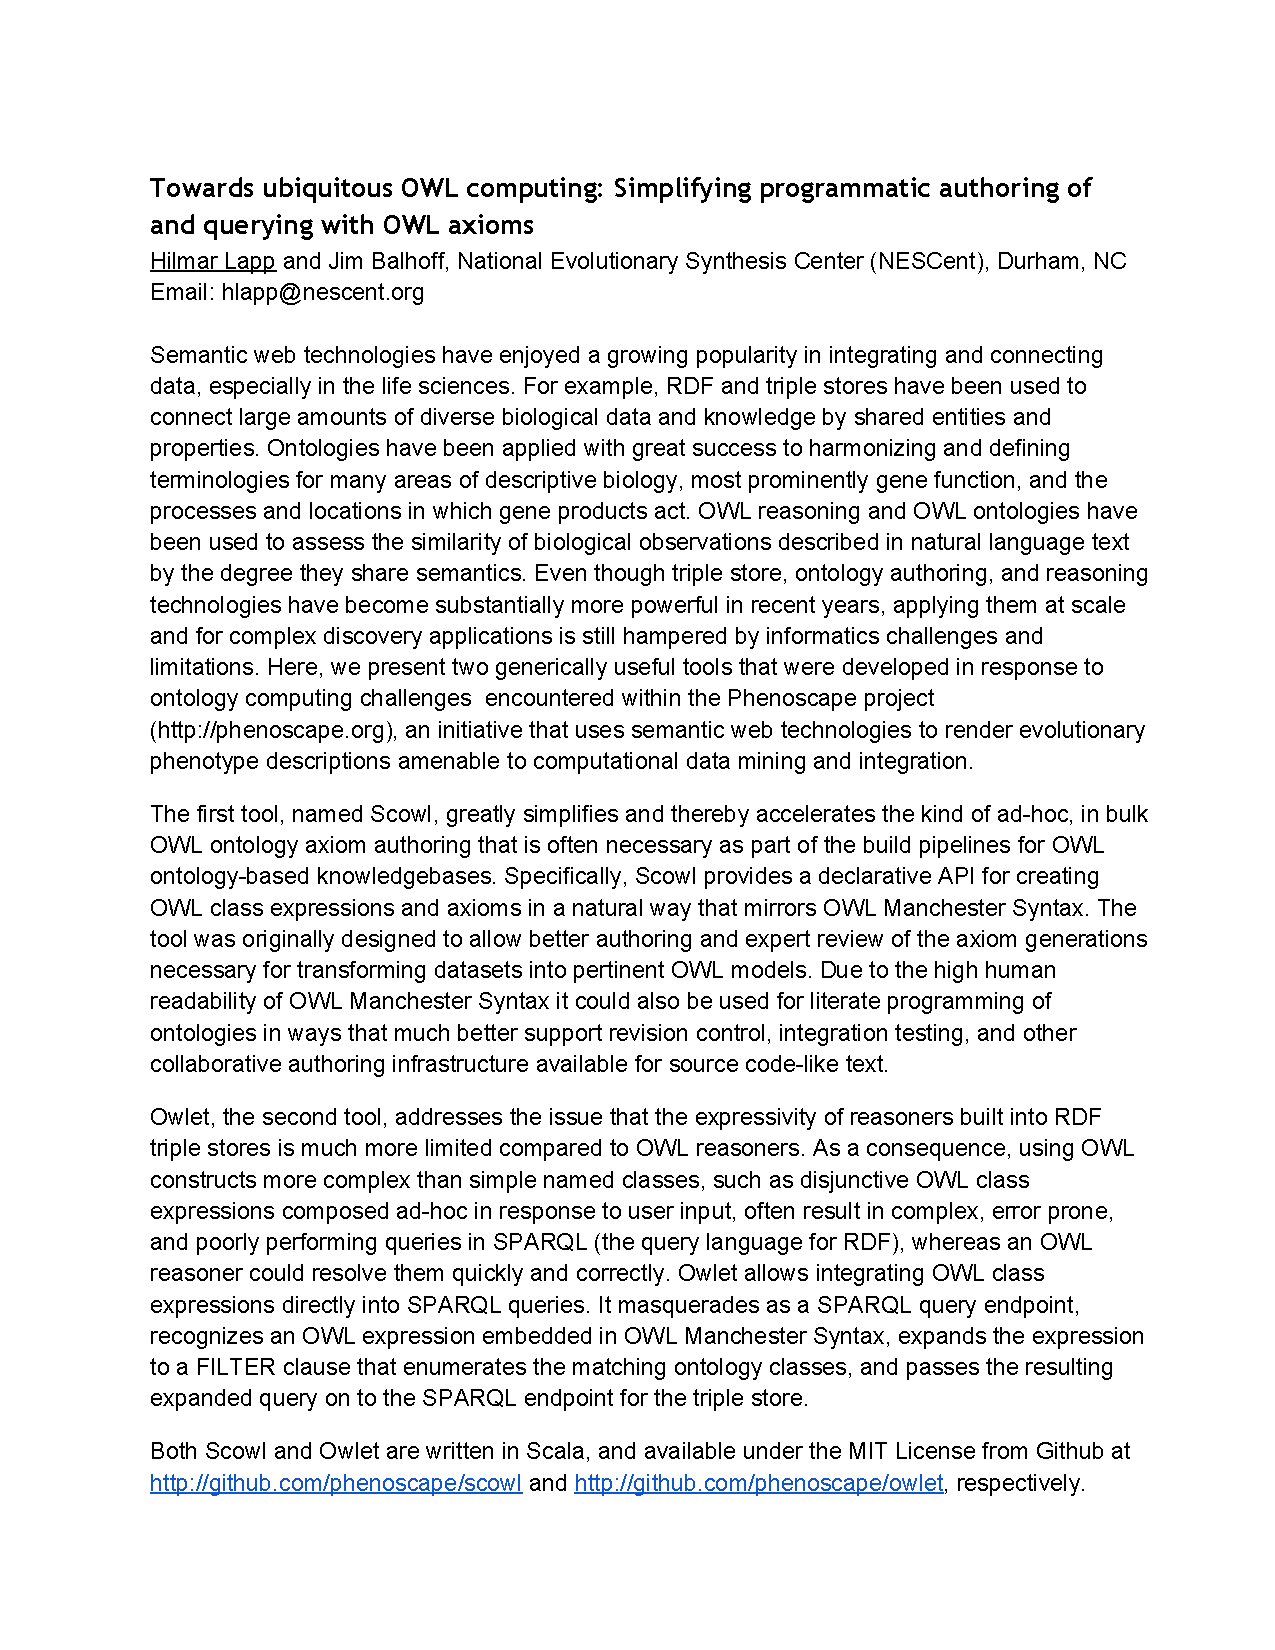
\includepdf[pages={1}]{Interoperability-34-OWL-computing.pdf}
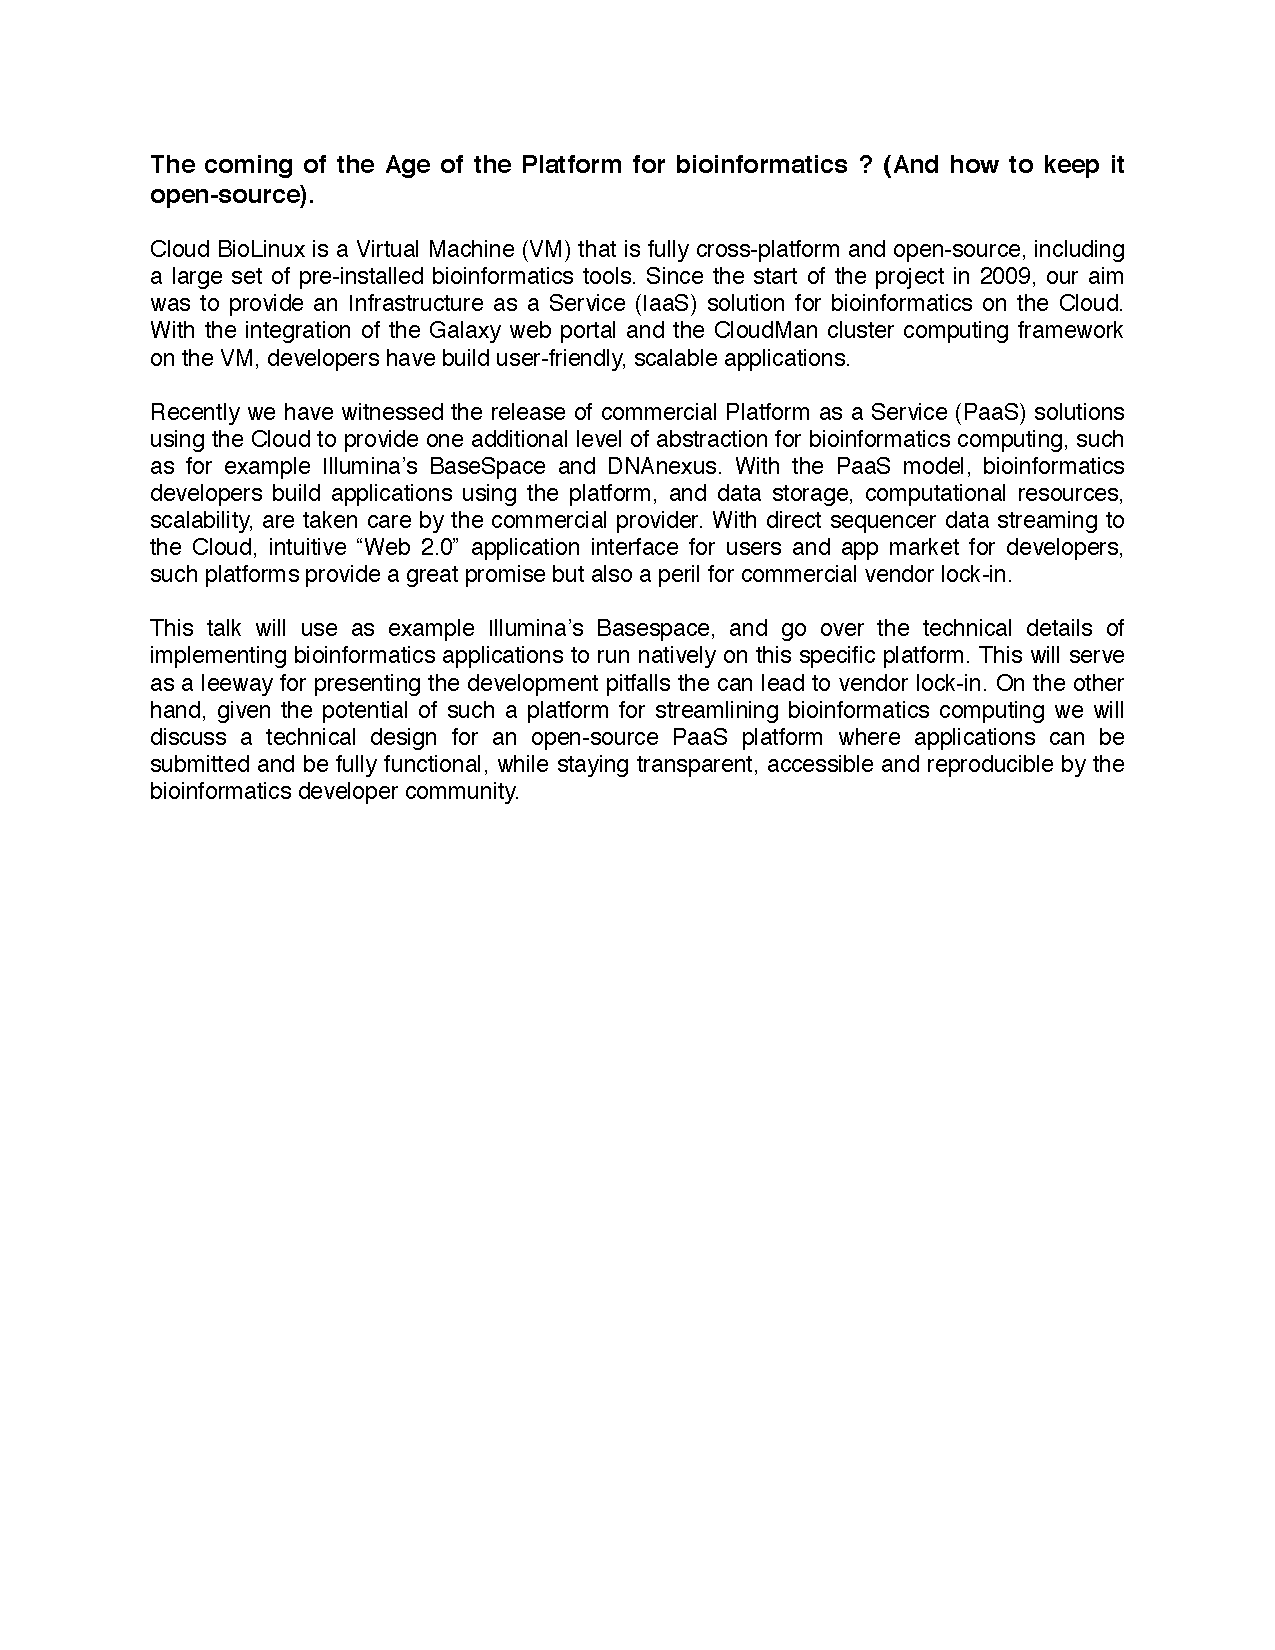
\includepdf[pages={1}]{Ineroperability-29-Age-of-platform.pdf}
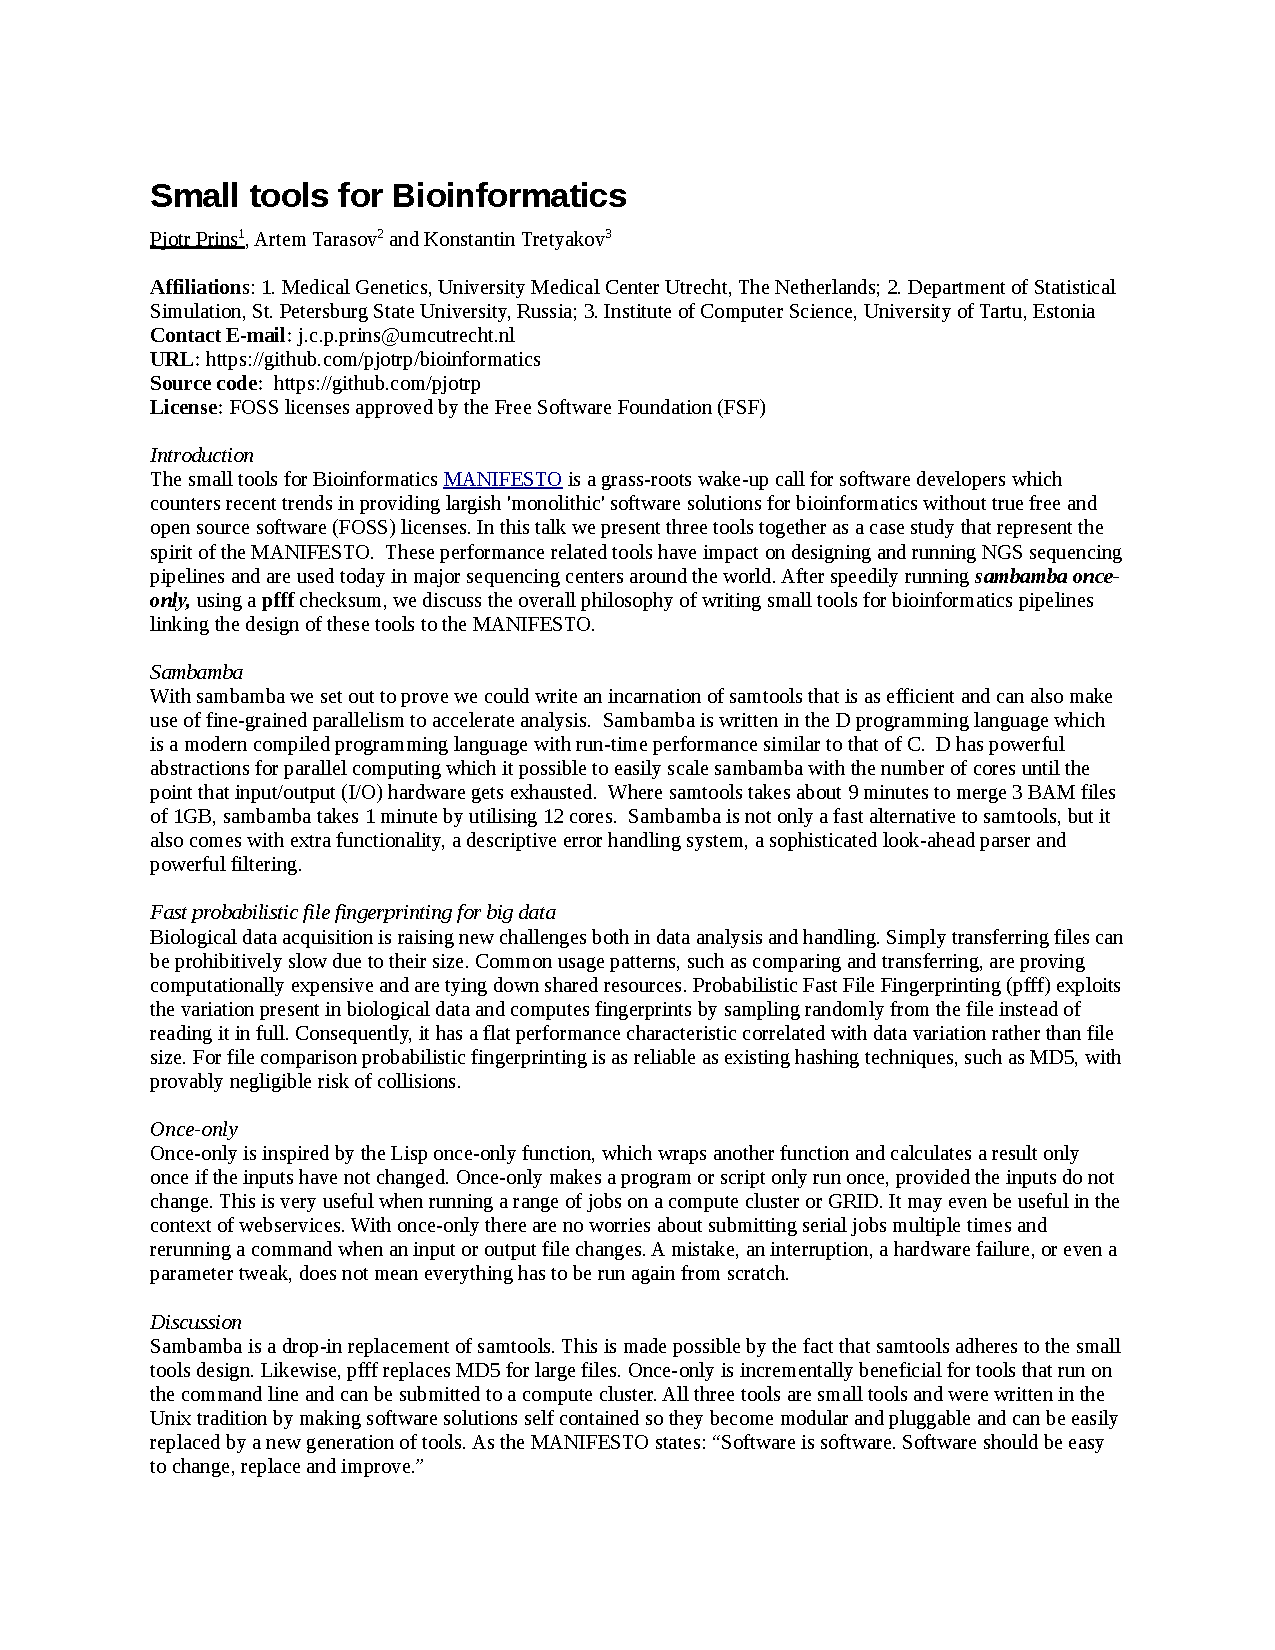
\includepdf[pages={1}]{Ineroperability-40-Small-Tools.pdf}

\newpage
\section*{Open Science and Reproducible Research }
BOSC 2014: Day Two, 11 July 2014, afternoon session 14:00 -- 15:30, and 16:00-16:15. \\
\noindent Number of talks: Five (5) plus one (1) after break before panel. \\
\noindent Session chair: Hilmar Lapp
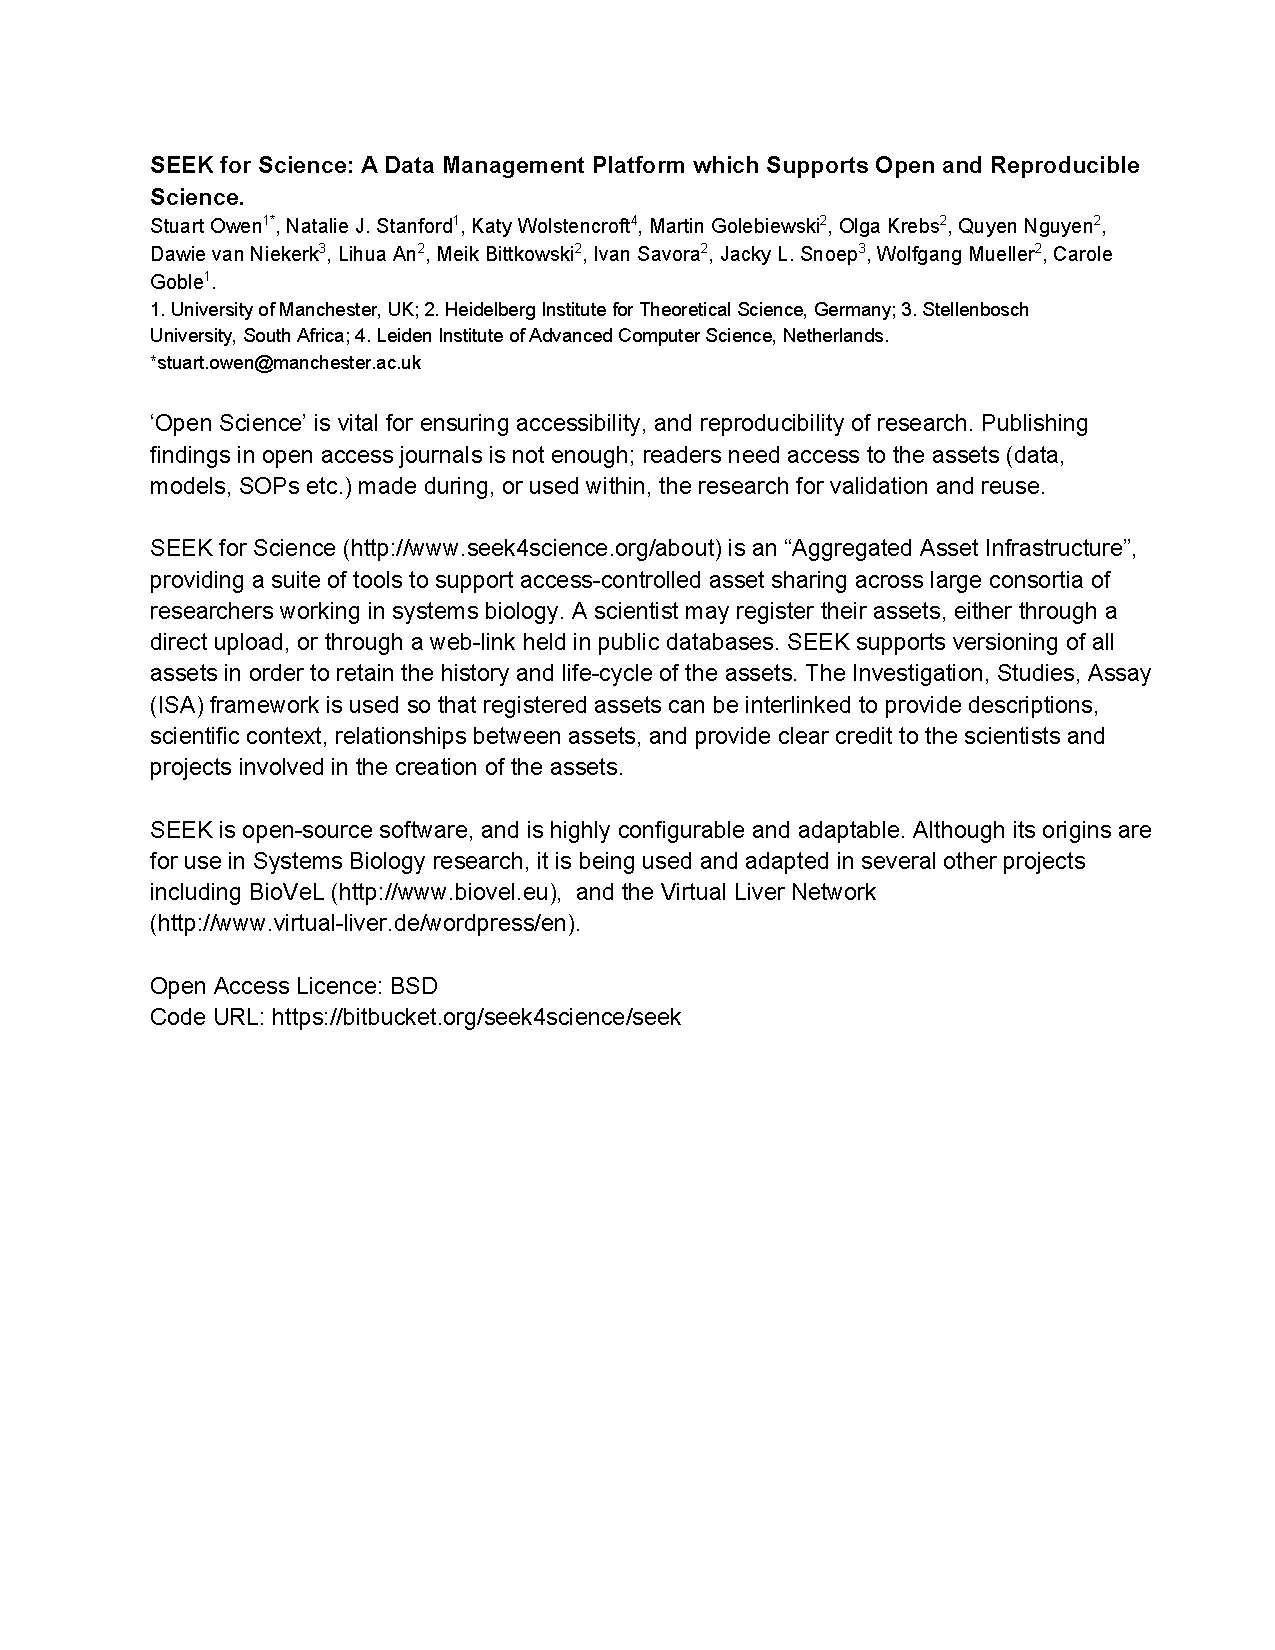
\includepdf[pages={1}]{OpenScience-11-SEEK.pdf}
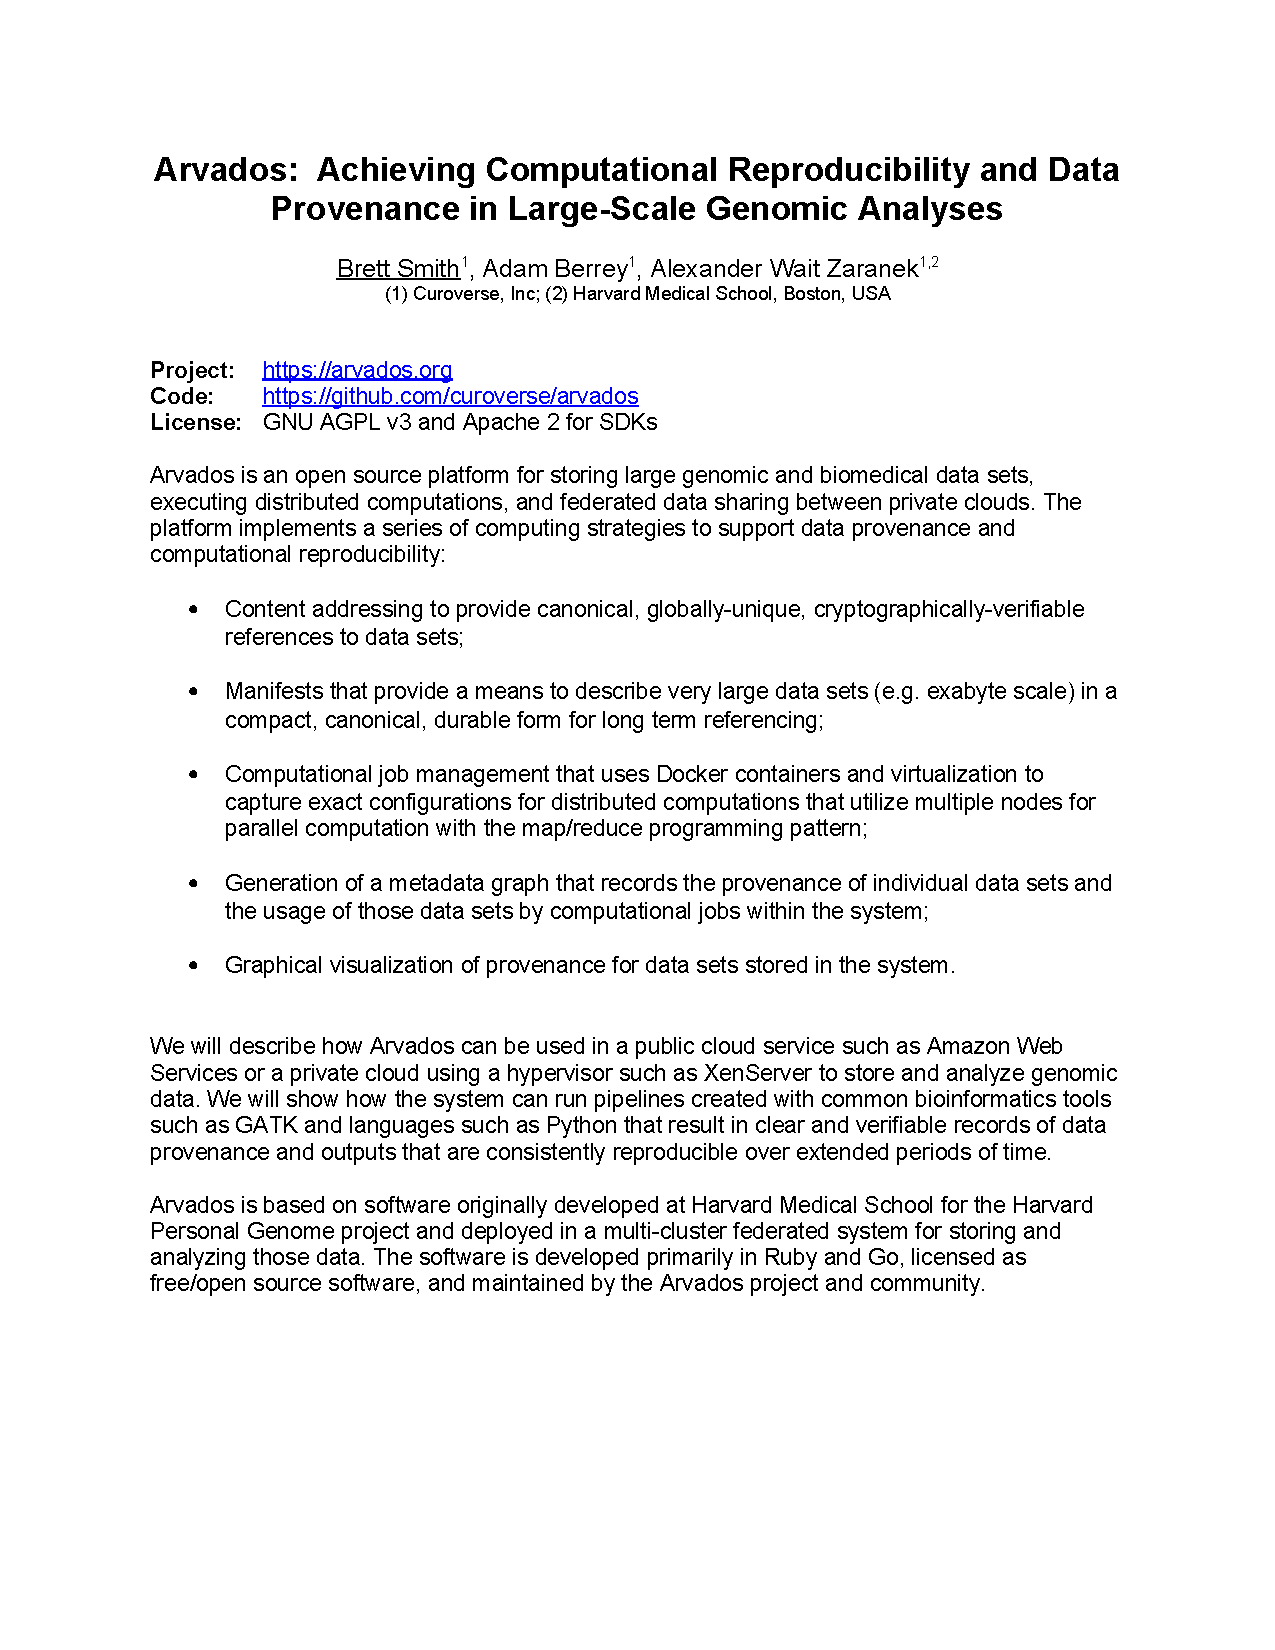
\includepdf[pages={1}]{OpenScience-31-Arvados.pdf}
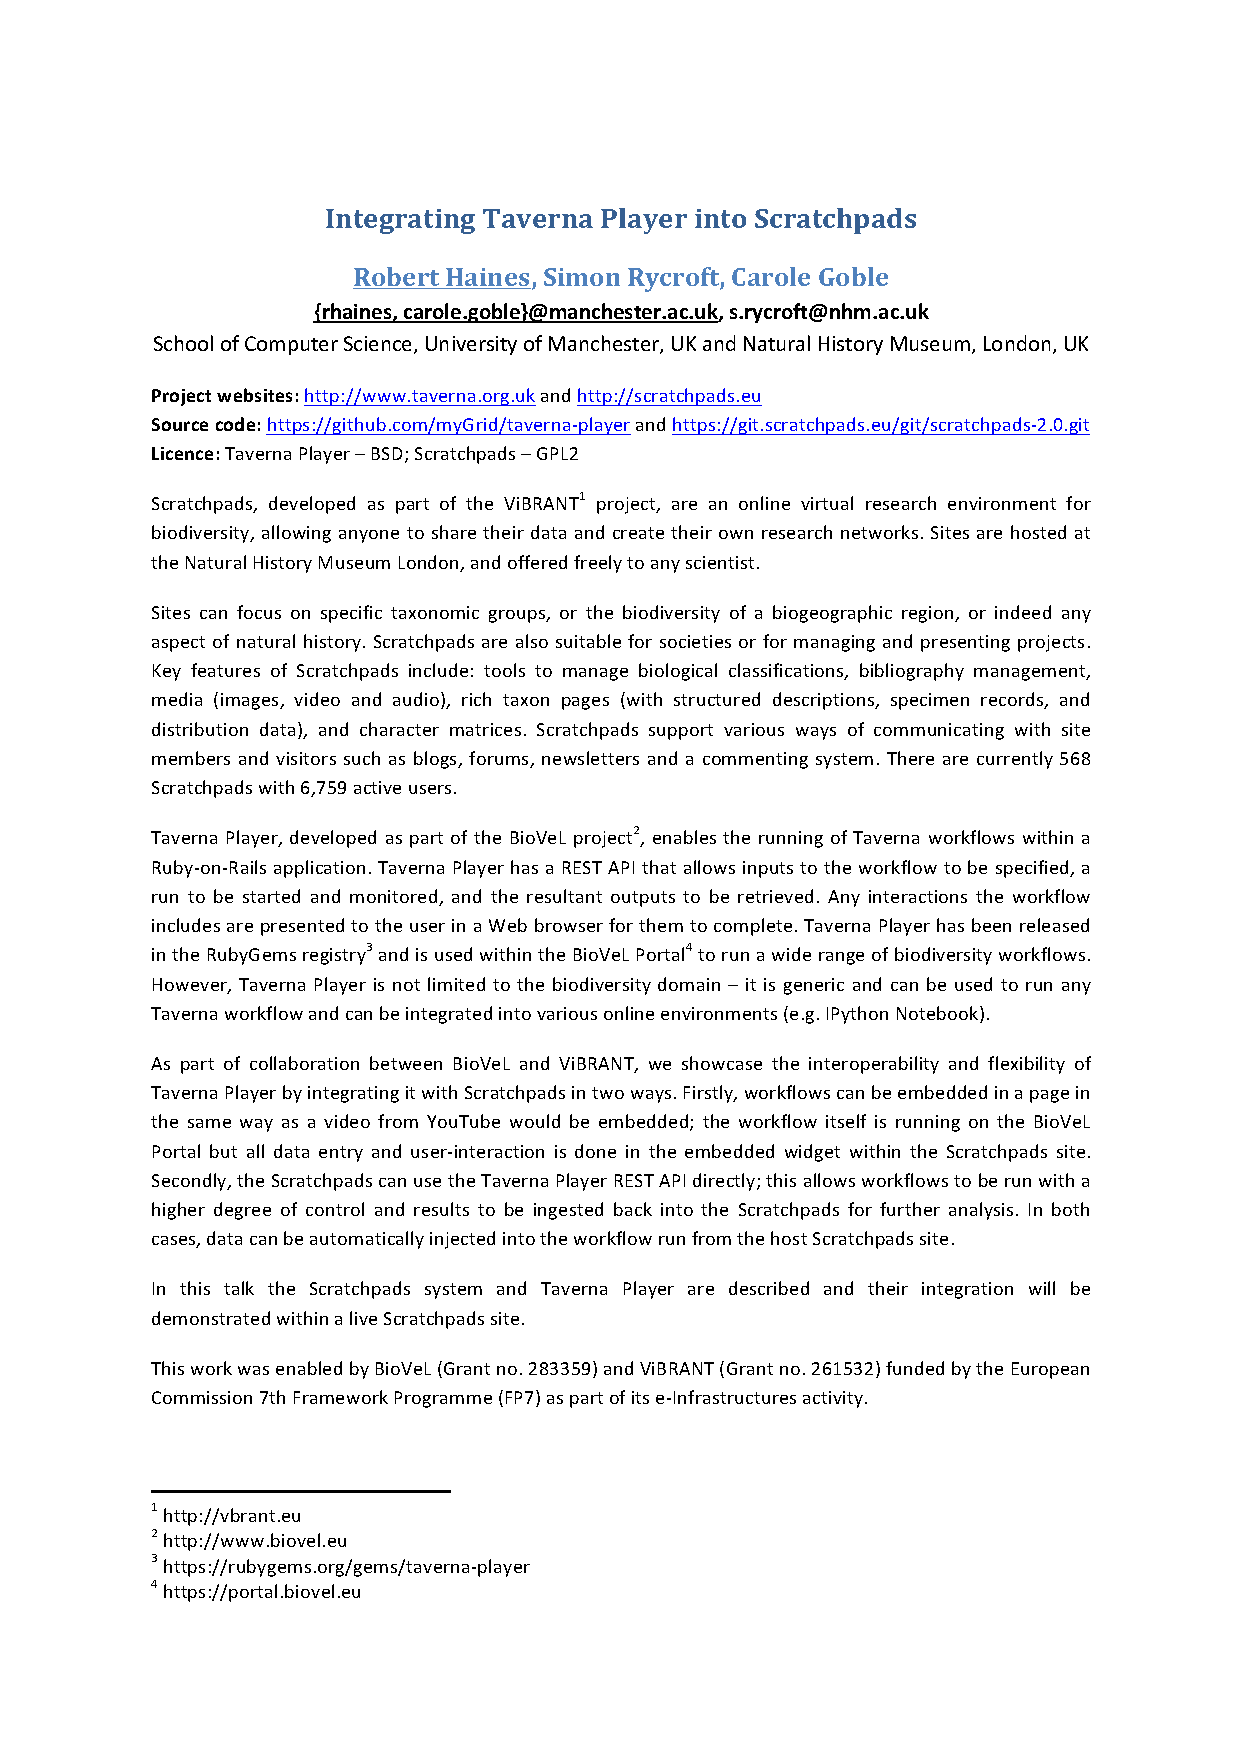
\includepdf[pages={1}]{OpenScience-14-Taverna-player.pdf}
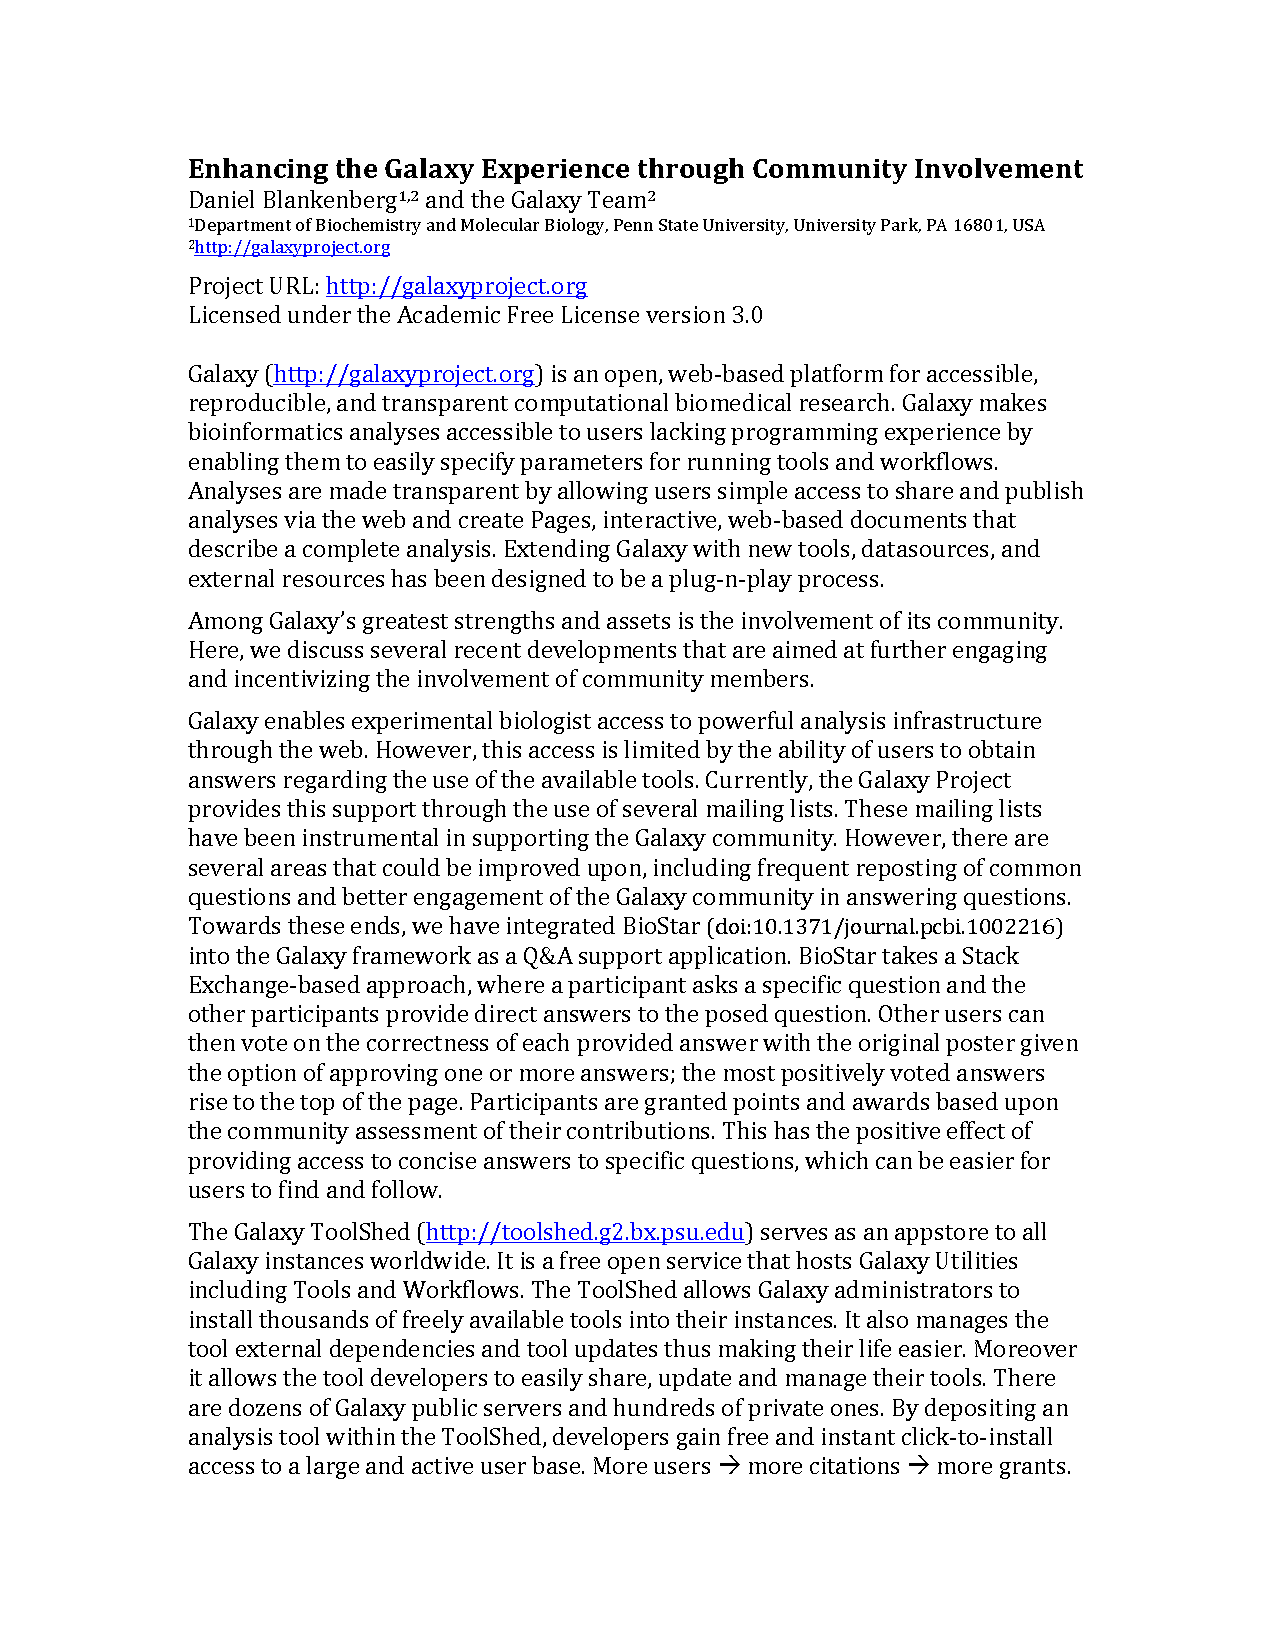
\includepdf[pages={1}]{OpenScience-35-Galaxy-community.pdf}
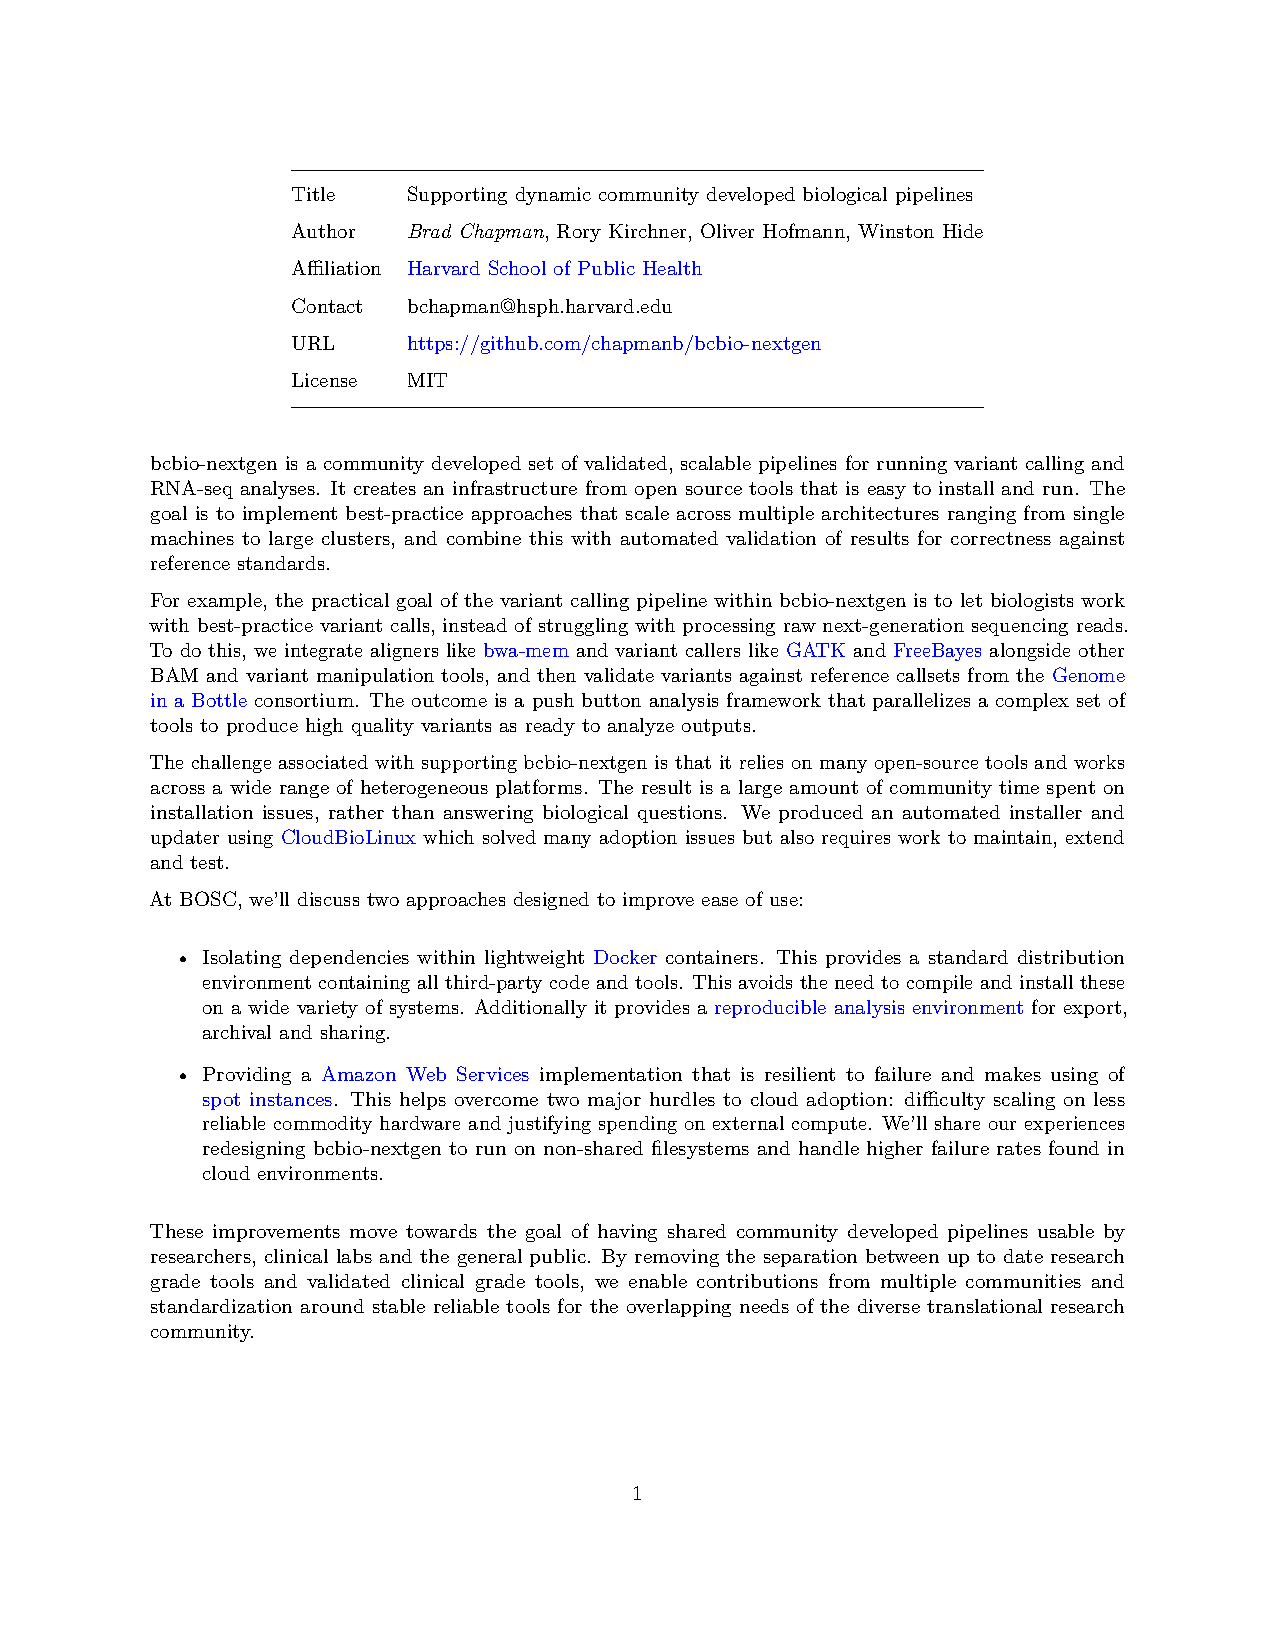
\includepdf[pages={1}]{OpenScience-23-Community-Pipelines.pdf}
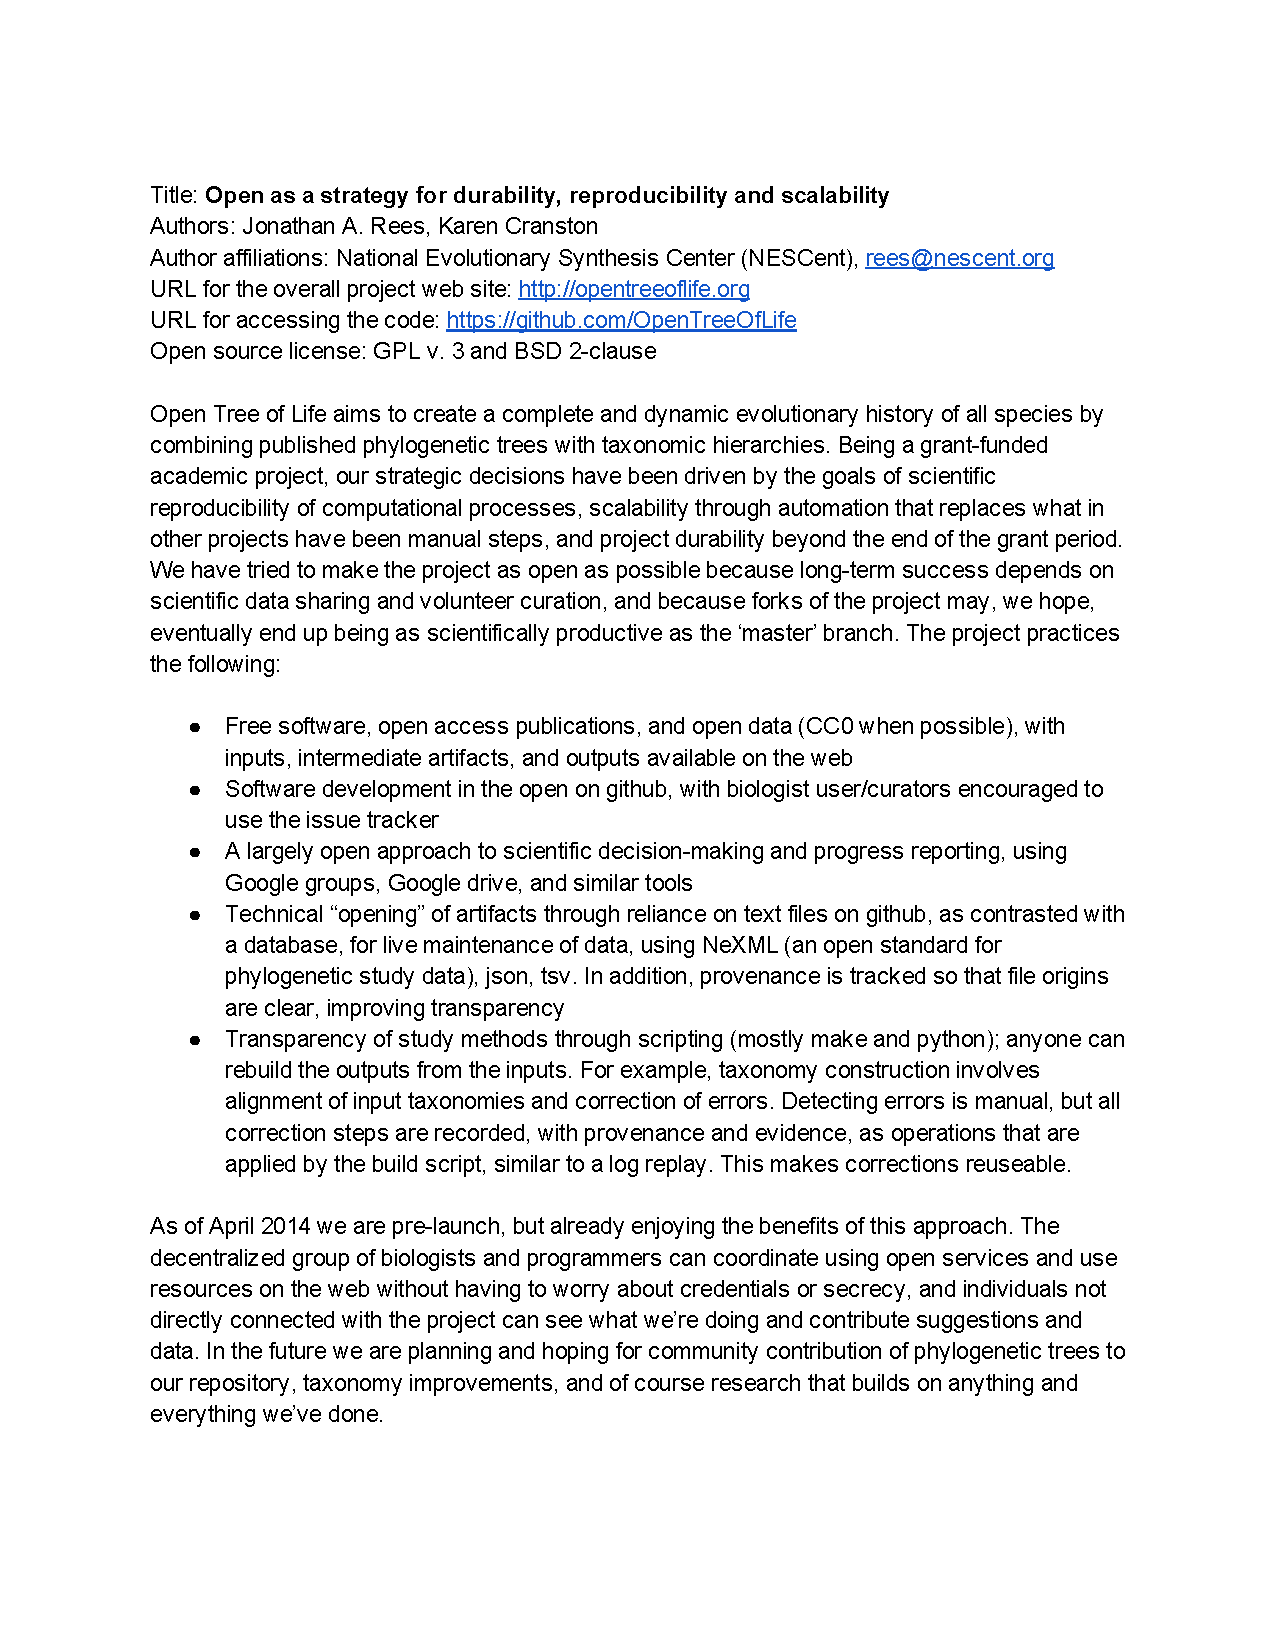
\includepdf[pages={1}]{OpenScience-26-Open-Tree-of-Life.pdf}

\end{document}